%************************************************
\chapter{AtomicOrchid Study 1: Non agent version}\label{ch:mathtest} % $\mathbb{ZNR}$
%************************************************
In this study, we focus on investigating requirements for time critical distributed team support relevant for domains such as disaster response. In this Field responders of the AtomicOrchid game use smartphones to coordinate, via text messaging, GPS, and maps, with headquarters and each other. Interaction analysis is conducted to examine log data and field observations revealing local and remote coordination within the responder team. We generate design implications for HACs system to support team coordination and uncover requirements that highlight the role of local coordination, decision-making resources, geospatial referencing and message handling. \\


\section{Introduction}
Disaster response (DR) has been characterised as highly coordinated, time-critical collaborative activities  \cite{Mendonca2007}. Coordination is essential in such settings so that time critical interdependent activities such as search and rescue can be completed in a timely and satisfactory manner \cite{Bradshaw2011}. Opportunity space for building `intelligent' coordination support for  such activities has been recognised by the researchers of HACs systems (see chapter \ref{ch:introduction}). However, little study has explored the  design space for HAC systems to support time-critical coordination settings. Therefore, little is known about the challenges and requirements in building systems to support team coordination in such settings.\\

Due to the critical nature of the disaster operations, it would be hard to design and deploy `intelligent' coordination in the field before we thoroughly explored the requirements of interaction design. On the other hand, computational simulation of an `intelligent' system is fundamentally insufficient for studying interactional issues (see section \ref{sec:interactional}). Therefore, in this study, we are aimed to use AtomicOrchid game as a game probe to uncover the requirements and design implication for building `intelligent' coordination support system. \\

The AtomicOrchid game creates socio-technical setting in which player teams plan and executes spatially distributed tasks (see section \ref{sec:sociotech}). Although HACs researchers has envisioned that an intelligent agent can team coordination by providing computational optimised task allocations in real-time, we focus on a base version of AtomicOrchid which does not involve any agent support in study. The aim is to unpack how human teams coordinate in the time and space constrained task setting, establish baseline performance of human coordination in the game, generate design requirements and implications for HACs systems, which in turn, supports our later system prototyping and studies. \\

This study is the first of three iterative system trials in this PhD work. The non-agent trial supports the two later (chapter \ref{ch:studytwo}, \ref{ch:studythree}) agent-supported system trials by 1) Revealing baseline performance of human coordination without agent support 2) Generate design requirements which feeds into subsequent prototyping of AtomicOrchid. The requirements are critical in that 1) the later studies can use them to recognize non-agent related design factors and 2) It also can inspire the interaction design between agent and responders in later system prototyping.  \\

In the following section, we will go through AtomicOrchid system description with a focus on interface and interaction design.\\

\section{System Description}\label{sec:system1}
% ===== how do I split this with Approach chapter
Basic game mechanic and system architecture has been introduced in the chapter \ref{ch:approach}. This section will give a detailed description of the system interface that support coordination between the field responders and headquarters players. \\

% the HQ interface 
The HQ is manned by two coordinators. All of the coordinators are provided with a web-based coordination interface (see figure \ref{fig:HQinterface}). The interface gives them an overview of the game status and enable them to communicate with the field responders. \\

% insert image here.
\begin{figure}[h]
  \centering
  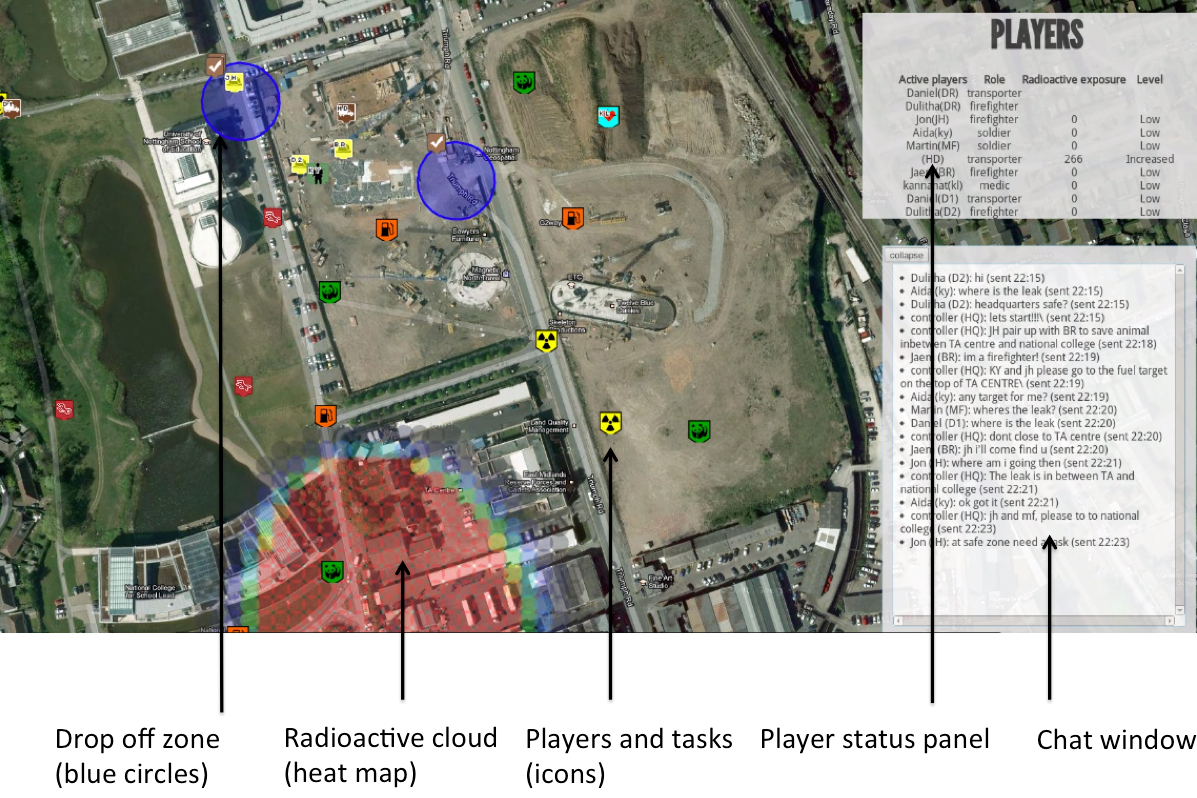
\includegraphics[width=1\textwidth]{img/study1/webinterface}
  \caption{The HQ interface}
  \label{fig:HQinterface}
\end{figure}

As you can see in the figure \ref{fig:HQinterface}, the majority space of the interface is occupied by a map-based presentation of the game status. Roles and locations of field responders are represented on the map as icons. The field responders can be uniquely identified by their initials shown on the icons. The target types and locations are also shown as icons on the map. Location and intensity of radioactivity is indicated by a heatmap. Heath status (health value ranges from 0 to 100) of the field responders is displayed on the right-top panel. A chatbox is placed on right bottom for HQ to browse and send messages. The messaging system follows a broadcasting model. Everyone can send messages to one public channel, and the messages are visible to every play through the mobile and HQ interface.\\

Field responders are equipped with a mobile responder app providing them with sensing and awareness capabilities (figure \ref{fig:mobileResponderApp}). There are two tabs in the responder apps. The "map" tab displays a map showing locations of field responders and targets, which is similar to the map on HQ interface, except that the radioactvity is not shown. The radio level of players' current location is displayed as a Geiger counter reading (shown as a number on the top left of the screen ), which ranges from 0 to 100. Health status of the field responder is indicated by a health bar on the right side of the Geiger counter. The chatbox (similar to the one on HQ interface) is placed on the "Messages" tab for field player to receive and send messages.\\


% the mobile responder app
\begin{figure}[h]
  \centering
  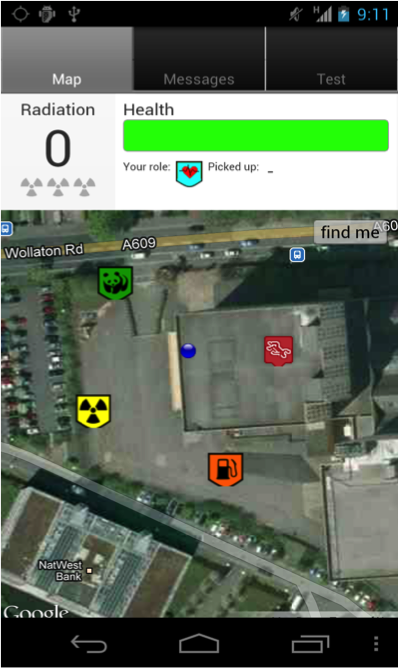
\includegraphics[width=0.5\textwidth]{img/study1/mobileinterface}
  \caption{The mobile responder app}
  \label{fig:mobileResponderApp}
\end{figure}

% move this to the study 1 chapter. 
 The app shows a reading of radioactivity, their health level based on radioactive exposure, and a GPS-enabled map of the game area with the targets to be collected and the drop off zones for the targets. Icons according to responder roles that additionally have their initials on them can be used to identify individuals. Another tab reveals the messaging widget to broadcast messages to the other field responders, and to headquarters.\\



\section{Study Design}

% ====== checked from COOP, should be fine =======

To explore socio-technical issues around team coordination, we ran two Radiation Response Game sessions, with volunteers recruited from the local university. We describe participants, procedure, session configuration, and methods used to collect and analyse quantitative and qualitative data.\\

Study participants were recruited through posters and emails. A total of 18 participants were recruited (8 female); 7 participated in session A and 11 in session B. All participants were reimbursed with 15 pounds for 1.5 hours of study. The majority of participants were students of the local university. Procedure. Upon arrival in the HQ (set up in a meeting room at the local universi- ty), participants were briefed and asked to consent to participate. Roles were ran- domly assigned to all participants (HQ/field responders: firefighter, medic, trans- porter, soldier). Field responders were provided with a smartphone; HQ coordinators with a laptop. Game rules and interfaces were introduced, and partic- ipants were assisted in setting up their phones and laptop clients. Field responders and HQ coordinators were given 5 minutes to discuss a common game strategy. All field responders were accompanied to the starting point within the designated game area, about 1 minute walk from headquarters.\\

Once field responders were ready to start, HQ sent a ``game start'' message. Gameplay commenced for 30 minutes. A ``Game over'' message by HQ concluded the game. Field responders returned to HQ for the post-game session.The post-game session consisted of a questionnaire aimed at collecting participants` feedback on (1) first impressions of the game; (2) usability of the system,and; (3) coordination issues in the game. A group interview was then conducted, before participants were debriefed and dismissed.\\

The size of the game area on the local university campus was 400 by 400 meters, without heavy traffic. The terrain of the game area includes grassland, a lake, buildings, roads, and footpaths and lawns. There are two drop off zones and 16 targets. The pilot study showed that this was a challenging, yet not too overwhelming number of targets to collect in a 30 min game session. There were four targets for each of the four target types. The pattern of cloud movement and expansion was the same for both game sessions.\\

We took a mixed methods approach to data collection and analysis. In addition to quantitative questionnaires, a semi-structured group interview was conducted aimed at eliciting important decision points, strategies and the overall decision-making process. Furthermore, five researchers with camcorders recorded the game play. One researcher recorded action in the HQ, and four other researchers each recorded a field responder team.\\

We developed a log file replay tool to help with data analysis of time stamped system logs that contain a complete record of the game play, including responders` GPS location, their health status and radioactive exposure, messages, cloud location, locations of target objects and task status.\\

\textbf{Interaction analysis of local coordination} We focus on the analysis of local field responders` interaction to unpack team coordination, including handling of mes- sages sent by HQ. Video recordings of field action were catalogued to identify sequences (episodes) of interest (cf. Heath et al., 2010). Key decision points in team- ing and task allocation served to index the episodes. Interesting distinct units of interaction were transcribed and triangulated with log files of relevant game activity for deeper analysis that we present in this paper.\\

\textbf{Message classification} How are remote messages used as a coordination resource? We used speech-act theory and the notion of adjacency pairs in linguistics to classify messages sent between and among responders and HQ.According to speech act theory, utterances in dialogues can be considered as speech acts from three dimensions. We were primarily concerned with the illocutionary dimension of speech acts. Searle`s classification of illocutionary acts (Searle, 1975) is used to categorize messages in the communication system.\\


\section{Data analysis and results}
Here, we present findings from interaction analysis supported by message classification that reveal how team coordination was achieved. Results of the message classification will be presented first, followed by detailed analysis of episodes. 

% this is from COOP paper, need to adapt it for this writing 
%{An overview shows that directives from HQ are frequently not brought up locally. A further episode demonstrates how field responders instead draw on technological and embodied resources to achieve local coordination, without HQ involve- ment. Finally, two more examples illustrate how responders routinely employ messages as a resource to support situational awareness.\\ %}

\subsection{Speech act analysis on text messages}
Overall, responders rescued 7 and 9 targets in session A and B respectively, out of 16 targets in total per session. Two players were incapacitated in session A, and 1 player was incapacitated in session B. 117 and 70 messages were sent in session A and B, respectively. We used Searle`s classification of speech acts to categorize messages (see table ref{fig:speachact}). We also add requests to the table to categorize all of the messages (Searle does not classify those as speech acts).\\

\begin{figure}[h]
  \centering
  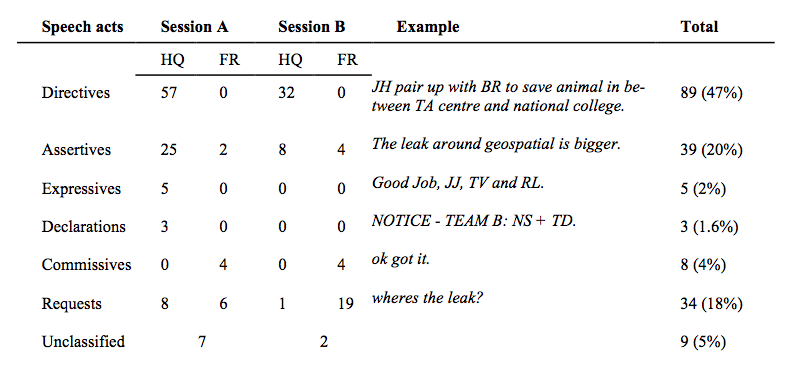
\includegraphics[width=1\textwidth]{img/study1/speechact}
  \caption{Speech act classification}
  \label{fig:speachact}
\end{figure}

\subsubsection{Directives}

Most messages in the category of directives are instructions sent by headquarter (HQ) players. The content of instructions can be related to two themes: task allocation and task execution. Therefore, we further categories the instructions into two categories: instructions for task allocation, and instructions for task execution. The purpose of task allocation instructions is to distribute plans to field teams and require them to execute it. Most instructions in this category follow a common pattern. Let`s take a look at the example below:\\

\begin{quote}
\texttt{``HQ : JH1 pair up with BR to save animal inbetwen TA centre and national college''}\\
\end{quote}

The instruction sent from Headquarter consists of two parts: (1) Description of Team- ing (who are involved) (2) Description of Location (Targets) to go.It is worth mentioning that HQ players use different strategies when they try to de- scribe a location to field players. HQ players in session D frequently referred to land- mark on the map in their description, while HQ in session C used simple directions (north, west, south east). For example:\\

\begin{quote}
\texttt{``HQ: TEAM A, can you head south to the radiation and animal targets? Instructions for task} execution''\\
\end{quote}

The purpose of task execution instructions is to help players execute their tasks after they have been assigned tasks. Most instructions in this category are related to radio- active cloud. To help field players avoid radioactive clouds, HQ players frequently send directions to field players or simply urge field players to move quicker. For example:

\begin{quote}
\texttt{``TEAM B you need to be quick''} \\
\end{quote}

\subsubsection{Assertives}

in this game, assertives provide plain information to recipients. Most assertives are sent by headquarter because they have access to critical information the cloud location. Followings are some examples of assertives:\\

\begin{quote}
\texttt{``the leak around nottingham geospatial is bigger''}\\
\end{quote}

\begin{quote}
\texttt{``HQ:There's another leak by the lake!''}\\
\end{quote}

Interaction analysis shows that assertives are important for field players maintain situational awareness. We will talk more about this shortly in the section `` awareness''.\\

\subsubsection{Commssives, expressives and declarations}
We also identified a small number of commissives, expressives and declarations. Commissvies are field player`s response to an assertive or directive. It can be an acknowledgement of receiving a piece of information or commitment to execute a plan. (e.g. ``ok got it'', ``I am heading there'' ). Expressives and declarations are only found in session C. Expressives are typically HQ`s congratulations to field players. (e.g. ``HQ:Good Job, JJ, TV and RL'' ) In session C, HQ players sometimes declare field players to be in a team (e.g. ``NOTICE - TEAM B: NS + TD''). The declaration helps HQ to refer to a team easier.\\

\subsubsection{Requests and Adjacency pairs}
In linguistics, adjacency pair is a term to describe conversational turn taking. The pairs can be question->answer, inform -> acknowledge, offer ->acceptance et al.For simplicity, we ignore the typology of adjacency pairs and treat all pairs as re- quest-> response. Any utterance that expects a response is considered as a request. We found a number of requests sent from Headquarters and field players (14 in session A and 20 in session B). Those requests can be related to a number of themes.\\

Field players may send request for: \\

\begin{enumerate}
\item Task assignment (e.g. ``anything for us to do'')
\item Teaming (e.g. ``firefighter with me for fuel?'')
\item Information about the cloud (e.g. ``wheres the leak?'')
\end{enumerate}

For headquarters:\\

\begin{enumerate}
\item They may ask idle players to respond (e.g. ``fighter who is free now?'')
\item They may request for acknowledgement (e.g. ``HQ:firefighter, respond'' )
\end{enumerate}

In comparison, only a small number of adjacency pairs are found in both sessions (8 in C and 8 in D), which means not all requests are responded. (see figure \ref{fig:adjacencypairs})

\begin{figure}[h]
  \centering
  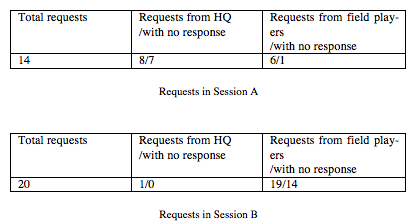
\includegraphics[width=1\textwidth]{img/study1/adjpairs}
  \caption{ Adjacency pairs}
  \label{fig:adjacencypairs}
\end{figure}

It is also worth mentioning that field players didn`t send acknowledgements to directives from headquarter. Although we do not classify directives as a request which expect an answer, the headquarter players express their frustration for not having response to their instructions. A HQ player said in the group interview:\\
\begin{quote}
\texttt{``I guess they did not look at it, they could not respond it, we were like saying ``where are you, respond'', but they did not respond. I guess they are busy seeing themselves and the targets''}
\end{quote}

A field players also commented on the issue:\\

\begin{quote}
\texttt{``I almost would not use the communication system because I was too focused on trying to save the targets.''}
\end{quote}

\begin{quote}
\texttt{``Sometimes I check whether the radiation is close to us, but mostly the communication is between us (local team members)''}
\end{quote}


\subsection{Responding to directives from HQ}
% TODO introduce episode 2 in my part as a simple unproblematice case here!!

We examine how field responders deal with messages from HQ that attempt to allocate tasks and manage task execution (i.e., directives). Classification of messages showed that directives were exclusively sent by HQ, and that they were the most frequent kind of message (see fig \ref{fig:speachact}). Directives index (attempted) instances of remote coordination of field responders by HQ. The observed response to messages is critical to understanding relation- ships between local and remote coordination. The following episode depicts a team of three on their way to pick up fuel. Their path is blocked by radiation. Without a team, firefighter JH (on the left) has just joined soldier KY (on the right), and firefighter D2 who have just been allocated a task in a message by HQ. (see figure \ref{fig:study1ep11})\\

\begin{figure}[h]
  \centering
  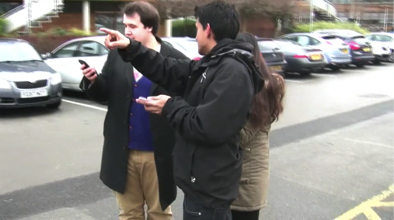
\includegraphics[width=.7\textwidth]{img/study1/ep1/ep11}
  \caption{JH (Behind Left), D2 (Middle Front), KY (Right behind)}
  \label{fig:study1ep11}
\end{figure}

\hfill \break
\noindent\Mybox{\begin{minipage}[b]{\textwidth}

\texttt{\textbf{KY:} ((reading out message)) KY and D2, please walk fast to the junction and quickly return back ((laughs))\\
\textbf{D2:} Oh is that what we have to do? Ok so we have to run to (2.0) We need to work out where we have to run to first and then get (.) get it back. Which junction is that? If you run to the next (0.5) thing ((points)), and then come back (1.0) that would work (1.0) is it safer to go around?\\
}
\end{minipage}}

\begin{figure}[h]
  \centering
  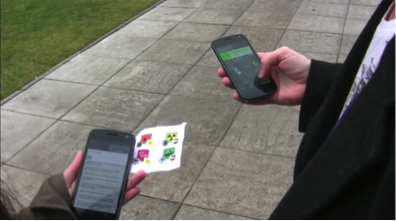
\includegraphics[width=.6\textwidth]{img/study1/ep1/ep12}
  \caption{KY (Left) , MF (Right) holding mobile phones}
  \label{fig:study1ep12}
\end{figure}


\hfill \break
\noindent\Mybox{\begin{minipage}[b]{\textwidth}
\emph{[The team tries to go around the cloud but is stopped by radiation, realising their target is in the cloud. Meanwhile, D2 has left due to increased exposure.]\\}
\texttt{
\textbf{KY:} So we have to run! [through the radiation] JH: Do we have to run through the (.) through the radiation? ((looking at map)) (see figure \ref{fig:study1ep12})\\
\textbf{KY:} Yah this is what the headquarters told us to do ((looking at messages)) (see figure \ref{fig:study1ep12})\\
\textbf{JH:} I have a terrible feeling thats gonna kill us.\\
\textbf{KY:} But its gonna be meaningful ((laughs))\\
\textbf{JH:} We go around this corner, if it gets to half [referring to health] we should probably start running back.\\
}
\emph{ [KY JH begin running into the cloud] } \texttt{(see figure {fig:study1ep13})}\\
\end{minipage}}



\begin{figure}[ht]
\centering
\begin{minipage}[b]{0.45\linewidth}

\includegraphics[width=1\textwidth]{img/study1/ep1/ep13}
\caption{Caption}
\label{fig:study1ep13}
\end{minipage}
\quad
\begin{minipage}[b]{0.45\linewidth}
 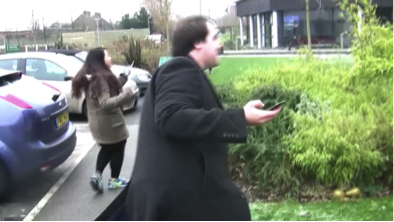
\includegraphics[width=1\textwidth]{img/study1/ep1/ep14}
\caption{Caption}
\label{fig:study1ep14}
\end{minipage}
\end{figure}

\hfill \break

\noindent\Mybox{\begin{minipage}[b]{\textwidth}
\texttt{
\textbf{KY:} ((yells)) OH OH! It`s a hundred! [refers to radiation level]\\
\textbf{JH:} We are basically in the middle of it! We are basically in the middle of it!\\
\textbf{KY:} ((shouts)) I`m going back? Get the fuel first! Get the fuel first! Oh no! \\
\textbf{JH:} We are not prepared for that! I blame our HQ.\\
\emph{ [They turn around and run back out of the cloud without the fuel.] } \texttt{(see figure \ref{fig:study1ep14})}\\
}
\end{minipage}} 
\hfill \break



This episode begins with a message by HQ attempting to help give directions to the target. D2`s response to the message is hesitant (is that what we should do?). His following question (which junction is that?) suggests the referent in HQ`s message is not understood. They attempt to go around the radiation. They realise their target is in the cloud. They refer back to the message to support their intent to go into the cloud to attempt to save the target (Yah this is what the headquarters told us to do). Having run into the cloud, they refer to the Geiger counter and realise the exposure is too high. Meanwhile, their health is decreasing rapidly. They abandon the task and flee to safety, whilst JH expresses his frustration (We are not prepared for that. I blame our HQ.).\\

First, the episode shows that geospatial referencing in messages can be problematic. It is unclear to the responders which junction HQ is referencing (and the responders do not ask for clarification), so they revise the route themselves. At the same time, they draw on the messages to justify their entering of the cloud. It does not occur to the responders that HQ allocated the task at an earlier time, before the cloud had covered the target. HQ does not update the responders on the increased danger, or revise their earlier task allocation. When the responder team fails to complete the task, they place blame instead of thinking self-critically.\\

Overall, out of the 43 task allocation directives HQ sent, the recipient field responders brought up only 15 messages in conversation in the team. The instances in which task allocation messages were addressed reveal the handling and value of HQ di- rectives in the local coordination. Firstly, out of the 15 task allocation messages responders talked about, they decided to ignore the instructions only once. The re- sponders ignored instructions because they were engaged in another task that they did not want to abandon. Secondly, four HQ instructions to rescue a certain target coincided with the same plan that had already been made locally by the respond- ers. In 10 cases, field responders chose to follow the instructions. However, due to confusion and misunderstanding they failed to follow them correctly six times. In fact, only 2 instances of directives from the HQ led to task completion. For the remaining 14 saved targets, field responders had locally allocated the tasks without HQ. (see figure \ref{fig:intructions})\\

% ===== insert the diagram from the JCSCW paper not COOP
\begin{figure}[h]
  \centering
  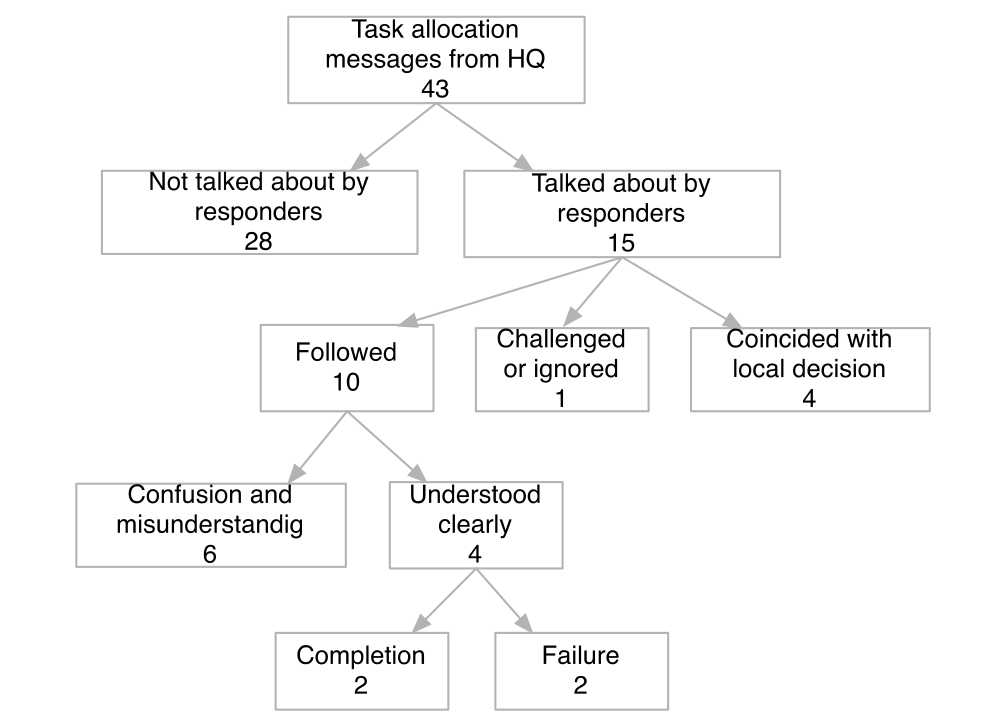
\includegraphics[width=1\textwidth]{img/study1/instructions}
  \caption{How responders addressed task allocation messages from HQ.}
  \label{fig:intructions}
\end{figure}

\subsection{Local coordination without HQ}\label{sec:s1localcoordination}
As presented, field responders predominantly coordinated teaming and task allocation of targets that were saved without HQ involvement. The following episode illustrates how field responders achieve coordination of teaming and task allocation locally. We join the action as BR and an- other responder are waiting at the drop-off zone without a compatible teammate, as MF and his teammate join and drop-off their target.\\

\begin{figure}[ht]
\centering
\begin{minipage}[b]{0.45\linewidth}

\includegraphics[width=1\textwidth]{img/study1/ep2/ep21}
\caption{Caption}
\label{fig:study2ep21}
\end{minipage}
\quad
\begin{minipage}[b]{0.45\linewidth}
 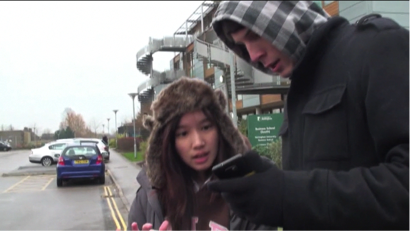
\includegraphics[width=1\textwidth]{img/study1/ep2/ep22}
\caption{Caption}
\label{fig:study2ep22}
\end{minipage}
\end{figure}

\hfill \break
\noindent\Mybox{\begin{minipage}[b]{\textwidth}
\emph{(on the right) and teammate walking towards BR (center)]\\}
\texttt{
\textbf{BR:} Any soldiers?\\
\textbf{MF:} I am soldier yeah.\\
\textbf{BR:} Would you like to pair with me? (2.0) to rescue a fuel?\\
\textbf{MF:} what are you after?\\
\textbf{BR:} I am a firefighter.\\
\textbf{MF:} Soldier and firefighter is fuel isn`t it?\\
\textbf{BR:} yeah.\\
\textbf{MF:} What can we get? (2.0) ((looks at screen)) this one in the center? ((points at screen))\\
\textbf{BR:} ((glances MF`s screen)) I think there are two people (the team D2,KY) going for that. I think we should go for this one ((points at screen)).\\
\textbf{MF:} We are going to get killed ((both laugh)).\\
}
\emph{[The team begins walking to target.]}\\
\end{minipage}} 

At the beginning of the episode, MF met BR, who was waiting at the drop-off zone without a compatible teammate. BR requested to team up with MF (``Would you like to pair with me? (2.0) to rescue a fuel?'') after MF identified himself as a soldier. BR and MF can then be observed sharing the screen of his device and using the map to identify potential targets. They realise one of them is already being pursued by another team. They agree on another target to pursue. Note that messages do not play a role in this episode. It exemplifies how teaming and task allocation are achieved locally, without consulting HQ. \\

The next episode is a follow-up episode, which demonstrates how two teams resolve the conflict when they approach a same target.

\begin{figure}[h]
  \centering
  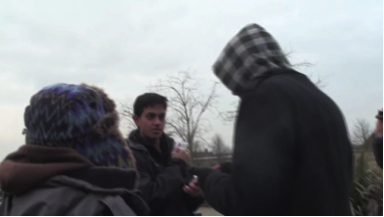
\includegraphics[width=0.7\textwidth]{img/study1/ep5/ep51}
  \caption{Caption}
  \label{fig:intructions}
\end{figure}

\hfill \break
\noindent\Mybox{\begin{minipage}[b]{\textwidth}
\texttt{
\textbf{D2:} we are told to get this fuel (target 1) from HQ.((pointing to screen))\\
\textbf{MF:} you are going to the fuel (target 1) we are aiming for, we thought you are going for this one (target 2).\\
\textbf{D2:} we were until we got a message saying not to. \\
\textbf{MF:} you get that one (target 1), we get that one (target 2).((pointing to the two target locations))\\
\textbf{D2:} if you want get that one (target 2). It is somewhere in the building.\\
}
\emph{[The two teams split, proceed with the new target allocations]}
\end{minipage}} 

At the beginning of this episode, the team (BR, MF) has decided to pursue (see ep x) a target other than the one pursued by team D2, KY. However, instructed by HQ, MF and KY changed their target and met BR and MF on the way. The two teams then began to show their intended targets to each other. After they find they are heading to a same target, MF suggest a new allocation of tasks (``you get that one, we get that one.''). D2 then offered some information about the target location to the team MF,BR (``if you want get that one. It is somewhere in the building.''), suggesting he agreed with the new task allocations proposed by MF. \\

The two previous episodes show that how teaming and task allocation are achieved in a ``ad-hoc'' manner. By using the word ``ad hoc'', we stress the the actions of field responders are typically not planned ahead adequately. The players often exchange information through conversations when co-located, and their plans are ready to be changed when new information is acquired. Take episode x as an example, while BR was waiting at the drop-off zone, she requested to team up with MF who happened to pass by. MF agreed to team up and then decided to aim for an available target that have not been aimed by others. In episode y, the two teams quickly came up with new task allocations when they found they were actually heading to the same targets . In the interview at the end of study, field responders also confirmed their ``ad-hoc'' behaviour in the interview:\\

\begin{quote}
\texttt{``Just save the closest target then just pair up and go to the other one'' }
\end{quote}

\begin{quote}
\texttt{``We just check, with that group, which target we can get. We see on the map to find the closet one we can get.''}
\end{quote}

% Add an episode from my part how the field responder resolve conflicts, suggest it is opportunistic. 



\subsection{Messages as a resource of situational awareness}
In the Radiation Response Game, field responders need to be aware of what other responders are doing, where the `danger zone' is (the cloud), and where it is likely to move. Awareness of each other`s actions helps responders avoid conflicts in planning, while awareness of the danger zone is essential to survive. The following episode illustrates how responders use messages as a resource to gain situational awareness.\\

The episode takes place towards the end of game session B. The radioac- tive cloud has grown so much that navigation in the game area becomes increas- ingly difficult. MF is with a group of five responders, two of which are carrying an animal. The cloud is blocking their way towards the drop off zone; they stop.\\

\begin{figure}[h]
  \centering
  
\includegraphics[width=.6\textwidth]{img/study1/ep3/ep31}
  \caption{Caption}
  \label{fig:study1ep31}
\end{figure}

\noindent\Mybox{\begin{minipage}[b]{\textwidth}
\texttt{
\textbf{MF:} ((reads message from HQ out loud)) There is another leak around Geospatial. (1.0) Which is Ah: so there`s a leak sprung up there. ((points)) Geospatial is like (.) that building right there. They say there is another leak. We should go all the way round (0.5) to the top left one, I think.\\
}
\end{minipage}}

MF brings up HQ`s message of the new leak, and suggests a route around the new cloud. The group ends up following MF`s route suggestion as a result. News of the new cloud, provided by HQ, enables the group to change their route to avoid danger. We commonly observed responders sharing information that provides situational awareness through face-to-face conversation. In the previous example, MF shared the message with a group of responders he was with already. The following example takes place between D2 and his teammate, as they are approached by JH, who is currently without teammate.\\

\begin{figure}[h]
  \centering
  
\includegraphics[width=.6\textwidth]{img/study1/ep4/ep41}
  \caption{Caption}
  \label{fig:study1ep41}
\end{figure}

\noindent\Mybox{\begin{minipage}[b]{\textwidth}
\texttt{
\textbf{JH:} Where are you guys heading? \\
\textbf{D2:} To get the fuel.\\
\textbf{JH:} Okay. The closest one to you? \\
\textbf{D2:} I believe so.\\
\textbf{JH:} Ya okay cuz I think the leak is somewhere near the other one and the army. [referring to building]\\
\textbf{D2:} Oh (.) which one?\\
\textbf{JH:} They sent a message saying its between territorial army center. D2: We are trying to get the one here ((points)).\\
\textbf{JH:} The closest one. Okay.\\
}
\end{minipage}} 


Making use of the map as he approaches them, JH asks the others to clarify which fuel they intend to pursue (the closest one to you?). He proceeds to inform the team that the ``leak is somewhere near the other one''. D2`s re- sponse (Oh, which one?) suggests they did not know this. In turn, JH elaborates on the location of the cloud, using an anonymous ``they'' to refer to the source of his information. ``They'' is likely to refer to HQ as they previously sent a message with the information of the cloud`s location. Conversational sharing of important information was a common resource responders employed to achieve and maintain situational awareness. However, requests for information were regularly not reciprocated with a response: out of 14 requests in session A, 8 were not responded upon; and in session B, 14 out of 20 requests were not responded upon.\\

\section{Performance implications}
This section will present broader concerns emerged from the game for the design of HAC systems that support team coordinationå.\\

\subsection{Division of labour between HQ and Field Responders}
Firstly, the HQ plays an important role in providing situational awareness to the whole team. As the game mechanic provides the HQ exclusive access to location of radioactivity, the HQ managed to provide informational messages about the radioactivity to field players. Field players are able to pick up the information and spread it to other field responders through face-to-face conversations.(see episode x) Although HQ attempted to organise task allocations directly (through directives), their attempts are often problematic.  Although the field responders did not get too much planning support from HQ, they naturally organise themselves into small teams and carry out tasks. As shown in episode x and y,  face-to-face conversation is vital for task and team organisation. We observed that co-located team members collectively make sense of the remote messages and game status shown on mobile screen. The decisions like choices of team, targets and routes are  predominately made through local conversations.\\

The pattern of division of labour between field responders and HQ indicates the weak role of remote coordination. The responder's choices of teams and targets seem to follow an ``ad-hoc'' manner as they heavily rely on face-to-face conversation , which can only happen when players are co-located. Despite some disruptions from communication channel (misunderstanding and confusions), field players always managed to find team-mates and avoid conflicts in their plans (e.g. pursuing the same target). [connect to situated planning by Lucy suchman]. However, the ``ad-hoc'' local coordination indicates the absence of the notion of resource optimisation, which is often the main concern of multi-agent coordination algorithm. In a sense, it opens opportunity for computational support, but it also highlights some potential challenges for such support system. \\

Firstly, it would be problematic if globally optimised choices conflict with the ``ad-hoc'' choices that are obvious for human field responders. As we can not assume either the agent or human choice will be always correct, we need to carefully design the interaction between human and agent to ensure that they can collectively reach an informed decision.\\

Secondly, there is a danger to impose an inappropriate ``work model'' (assumed by agent support) on the human team. For example, current division of labour between HQ and field responder suggest that field responders are comfortable with HQ being a supportive role (providing situational awareness). However, a centralized coordination algorithm may need to coordinate the whole team, requiring every players to follow top-down instructions to reach global optimum of resource allocation. In that case, the role of control room may need to change and it is unknown whether the change will disrupt or support natural human workflow.[] \\

\subsection{Enhancing remote coordination}
The heavy reliance on the local coordination can partly be a result of the lack of remote coordination support. In other words, local coordination is easier to achieve and can be seen as fallback of remote coordination. In a co-located setting, players can naturally make their actions observable and accountable to each other through conversations, body languages, gestures et al.[need to connect to data]  and organise coordination activities reflexively. However, in the remote setting, the natural accountability of their activities become opaque.\\

A set of functionalities including GPS/map sharing, broadcasting has been provided. We have observed players utilise the functionalities to make sense of other team members' actions (see section \ref{sec:s1localcoordination}) and act accordingly. However, coordination with remote players is still overall problematic which can be evidenced by frustrations related to remote communication (will be detailed in section \ref{sec:study1requirements}).\\

We suggest the future planning support should properly support remote coordination in a way that facilitate accountability among distributed team members. The next section discuss some detailed requirements of remote coordination support drawn from the field observations. \\

%{ The natural social order that employed by the team members to make sense of the task environment. Players are observed to constantly revealing to others their action and plans via face to face conversation. CSCW concern that Geo-spatial distribution distributed  hinders team member's attempt maintain accountability . The lack of response in the communication channel shows that. The form of communication in this study appears to be unable to support the team member's accountability. The missing of remote coordination and the weak role of HQ in the planning activities may indicate communication breakdown, which can also be confirmed by a number of observations of understanding and confusions in the communication channel (see x.x.x).\\From this perspective, the domination of local coordination . Some of the reasons? %}

\section{Design Requirements}\label{sec:study1requirements}
We now discuss the requirements for team coordination that emerged from the game. The embodied game probe embedded responders in a challenging setting. They needed to communicate effectively to make time critical decisions on teaming and task allocation, both locally in the field as well as remotely through messaging. Field responders physically engage and navigate the environment to perform tasks while maintaining awareness of risk and danger. The data reveals multiple challenges for team coordination involving communication and decision-making. \\

\textbf{Local decision-making} The study showed that teaming and task allocation were predominantly organised locally among field responders, in an ``ad-hoc'' manner, on- the-fly fashion. Despite the fact that headquarters attempted to coordinate task al- location remotely, few of these directives were brought to conversation locally. Only 2 out of 16 tasks that field responders completed were remotely allocated by HQ. Local decision-making needs to be supported by HAC systems that aim to support time-critical team coordination, and need to integrate capabilities to ena- ble team-wide sharing of the local decisions.\\

\textbf{Coordinate resources} While field responders made decisions on teaming and task allocation in a seemingly ad hoc fashion, game data reveals how field responders draw on resources to achieve situational awareness in order to coordinate successfully. A common understanding of the location and movement of the radia- tion cloud was achieved by sharing information from game messages verbally in a local group. Face-to-face talk was an essential resource for relaying information from the Mobile Responder App to teammates, such as radioactive exposure, oth- ers` whereabouts, task status, and other monitoring of the broadcast messages. Future HAC systems need to take into account that such coordinate resources are likely to be comprised of digital as well as embodied human resources. \\

\textbf{Geospatial referencing} The results show that geospatial referencing was problematic in various ways, particularly in directive messages sent to the field players. Participants had different levels of knowledge of the campus, which made understanding of landmark references uncertain. Some participants also struggled with making sense of north/south/east/west directions in relation to their current position and orientation. To deal with misunderstandings, players had to ask for clarification via messages or spend valuable time discussing the reference locally in order to understand it. Consistent with the findings of Toups et al. (2009), de- signers need to think carefully about how the presentation layer of HAC systems may be augmented with information that facilitates geospatial referencing (e.g., grids, labelling etc.) to facilitate human in addition to machine readability. Freshness of messages. Problems arose from erroneous instructions or otherwise out-dated messages sent to field responders. In one case HQ sent a message in which two players with non-compatible roles were instructed to team up. This was particularly costly, as the players attempted to team up, and lost valuable time until they realised the game mechanics barred them from forming a team.\\

\textbf{Freshness of messages} As demonstrated in one of the episodes, reading out-dated messages in a dynamically changing environment can contribute to responders taking dangerous actions that they believe to be safe, because they do not realise that the infor- mation is out-dated. However, in most cases, recipients managed to identify temporally irrelevant messages, and thus avoided following them.\\

To reduce confusion about message freshness, HAC systems should address these issues at the UI level, both for responders and for HQ. Develop functionality to flag messages as out-dated or retract incorrect messages. Up-to-date messages are particularly valuable. Thus, our findings support the use of fresh social media as a source of information for disaster response, despite problems that can arise with validation, because crowdsourced information will in many cases provide better coverage than official sources.\\

\textbf{Acknowledgement of messages} In most cases, field responders did not acknowledge or respond to messages sent by the HQ. This was particularly problematic for directives (task allocation), as task status and field responder compliance often had to be inferred by observing their location updates on the map. This consumed HQ attention, with negative impact on HQ`s overall work on state assessment and task planning. Observations in the field suggest that the physical demands (e.g., co-located team movement through terrain at speed) and cognitive demands to maintain situational awareness (e.g., monitoring of radioactivity and messages) are likely factors that explain lack of acknowledgement.\\

As a result, user interfaces that enable and encourage field responders to quickly acknowledge HQ messages, with minimum cognitive load, should be consid- ered for messaging in HAC systems in such high demand settings. For effective team coordination in disaster response, interface and workflow designs need to factor in cognitive load and task demands for effective information distribution.\\


\section{Conclusion}
The objective of the research presented here was to generate requirements for sup- porting time-critical team coordination. In particular, we focussed on a scenario in which responders coordinate role-based teaming and spatially distributed task al- location and execution using a real-time location and messaging system.\\

We presented the design and study of the Radiation Response Game as a mixed-reality game probe to investigate challenges for team coordination in a set- ting in which participants experience both physical strain through bodily activity, and cognitive challenge through time pressure and task complexity. We eschew high-fidelity simulations in favour of mixed-reality game probes as a platform for investigation of concomitant socio-technical issues: handling of mobile devices to communicate and maintain situational awareness (messaging, sensing, interaction, and display) intersect with face-to-face interaction, whilst the physio-cognitive challenges created through game mechanics and environment induce stress. We created a setting that allows exploring requirements to support team coordination of relevance to time-critical coordination domains such as real disaster response.\\

Findings from interaction analysis of field observations, triangulated with log files, reveal how field responders achieved coordination by drawing on local face-to-face conversation with fellow responders, and situational information provided by the interactive map, the Geiger counter, and the messages sent by HQ. Drawing on these findings, we generated requirements for supporting team coordination, emphasising the roles of local coordination, decision-making resources, geospatial referencing and message handling. These requirements inform future work on building human-centred HAC systems by emphasising the role of human interaction in team coordination in time-critical settings.\\

%************************************************
\chapter{AtomicOrchid Study 2: Agent supported HuOL design}\label{ch:studytwo} % $\mathbb{ZNR}$
%************************************************
This chapter presents the second iteration of AtomicOrchid field trials. In this study, a planning agent is integrated into the system by following a HuOL interaction design, in which the HQ only monitor and occasionally intervene the planning agent. The purpose of the trials is to investigate socio-technical issues relating to integrating the planning agent to rescue team with the HuOL interaction design. Interaction analysis is conducted to examine log data and field observations unfolding how human agent interaction plays out, which in turn, revealing the process by which players interpret and negotiate the agent guidance as well as how these are intertwined with social dynamics of the teams.

\section{Introduction}\label{sec:studytwointroduction}
Task planning in teams can be complicated by both spatial and temporal constraints, particularly in time-critical task domains such as disaster response (DR). In a DR setting, responder teams have to coordinate sparse resources and personnel to prioritize geographically distributed tasks, forming and disbanding teams dynamically to carry out DR operations [4]. Multi-agent researcher has devised a number of agent coordination algorithm to coordinate task allocations for multi-agent systems, which create opportunity for computational planning support for DR teams. \\

However, these algorithms typically model humans as computational agents with respective capabilities, for example to dynamically allocate teams of agents to tasks in order to maximise an objective (e.g., number of lives saved), taking into account other aspects of the real world (environment, infrastructures, victims, etc.) [14]. Therefore, the quality of the planning results can be constrained by limited assumptions of human behaviour (e.g., human psychosocial characteristics, movement, and learning ability)and real world environment [18]. These limitations highlight importance of human input in the planning process. Thus, we argue that effective collaboration between human and agent is required to produce and execute high quality plans in the disaster setting. (refer to background section?). \\

In other to support effective Human agent collaboration, a number of interaction design strategies have been identified, including design patterns such as HuOL and HuIL (see section \ref{sec:interactional}). In this study, the planning agent is integrated into the AtomicOrchid system with a straightforward HuOL design pattern. This interaction design pattern assumes minimal Headquarter intervention and simple feedbacks from field responders are required by the agent to perform task planning. The interaction design is aimed to facilitate the division of labour between humans and agent: a planning agent routinely assigns tasks to distributed responder teams, while human coordinators (the HQ) monitor and support the task execution by responding to arising contingencies. The agent is designed in a way to take into account simple human feedback, i.e., a field responder can either reject or accept their task assignment. The agent will consider the feedback for the next iteration of task assignment.\\

%insert figure

This study uses the agent integrated version of AtomicOrchid as a probe to unfold socio-technical issues in human-agent interaction, with focus on the implications of the HuOL design for human team performance. The implications for the interaction design are discussed that may improve team performance. More specifically, this chapter addresses the following research questions on how agent guidance affects the social organisation of team performance:\\

\begin{enumerate}
\item How do human teams respond to being instructed by an agent, particularly on switching teams and tasks?\\
\item The planning agent makes decisions based on limited assumptions about human behaviour, but what are the hidden costs of human behaviour that the agent does not take into account?\\
\end{enumerate}

Findings from the study highlight the social processes in which members interpret, negotiate, and manage the agent guidance within the social dynamics of teams. We discuss the division of labour between humans and teams; the hidden costs of instructions that suggest team reformation and interrupt on-going tasks. We conclude the paper with a number of emerging interaction design recommendations to consider when building agent-based support systems for human teams, which emphasise the need for common ground between humans and the agent, facilitate accountability between team members, and balance responsibilities between humans and the planning agent appropriately.\\


% ===== from CTS need adaptation =====
%We present a field trial of how instructions from an intelligent planning agent are dealt with by distributed human teams, in a time-critical task setting created through a mixed-reality game. We conduct interaction analysis to examine video recorded field observations and game log data. The findings highlight the social process by which players interpret and negotiate the agent guidance as well as how these are intertwined with social dynamics of the teams. The insights can be used to develop an understanding of interactional issues around automated team instructions and inform the design of human-centred planning support systems. \\

%Task planning in teams can be complicated by both spatial and temporal constraints, particularly in time-critical task domains such as disaster response (DR). In a DR setting, responder teams have to coordinate sparse resources and personnel to prioritize geographically distributed tasks, forming and disbanding teams dynamically to carry out DR operations [4]. For example, teams of fire fighters and medics are required to extinguish a fire and to provide first aid, while teams of soldiers and transporters may be needed to clear rubble. These teams, in turn, may need to disband and reform dynamically to perform new tasks and to adapt their planning to uncertainties in real time. Whilst an `optimal' plan of team formation and task allocation may help minimise loss of lives and properties, making optimal plans in real time can be complicated and time-consuming due to large numbers of incidents and responders. To address such coordination challenges, multi-agent research has developed a number of smart coalition formation algorithms to computationally support planning in time-critical task settings [3,16]. These algorithms typically model humans as computational agents with respective capabilities, for example to dynamically allocate teams of agents to tasks in order to maximise an objective (e.g., number of lives saved), taking into account other aspects of the real world (environment, infrastructures, victims, etc.) [14]. \\

%However, most of these smart algorithms are based on limited assumptions about human behaviour (e.g., human psychosocial characteristics, movement, and learning ability) [18], and have only been evaluated in computational simulations. In our work, we investigate agent-based planning support in the real world. Specifically, we study the social implications of the division of labour between agents and real human teams. In more detail, while coalition formation assumes leaving and joining new teams as an unproblematic process, we study in depth the social, interactional consequences of agent-based instructions that require team formation. For example, Personal preference and social norms may imply that dynamic team formations have a hidden social cost that may impact team performance. \\

%We present AtomicOrchid, a mixed-reality game probe of the ways in which human teams respond to agent guidance. The probe is designed to create a socio-technical setting in which distributed teams and a planning agent work collectively to save locally dispersed targets on the ground. The planning agent runs a coalition formation algorithm to help allocate tasks optimally to the teams. Our analysis reveals social implications of agent support for human teams. In turn, implications for interaction design are discussed that may improve team performance. More specifically, this paper addresses the following research questions on how agent guidance affects the social organisation of team performance:\\

%How does division of labour play out between humans and agents and how should it be scaffolded by design? 
%How do human teams respond to being instructed by an agent, particularly on joining and leaving teams?
%The planning agent makes decisions based on limited assumptions about human behaviour, but what are the hidden costs of human behaviour that %the agent does not take into account?\\

%Findings from the study highlight the social processes in which members interpret, negotiate, and manage the agent guidance within the social dynamics of teams. We discuss the division of labour between humans and teams; the hidden costs of instructions that suggest team reformation and interrupt on-going tasks. We conclude the paper with a number of emerging interaction design recommendations to consider when building agent-based support systems for human teams, which emphasise the need for common ground between humans and the agent, facilitate accountability between team members, and balance responsibilities between humans and the planning agent appropriately. 

\section{System Evolution}
Compared to study 1, the system has evolved to provide agent planning support through HuOL interaction pattern. This section will go through the changes of system, which includes integration of a planning agent, implementation of a quick feedback system, and improvement in both HQ and mobile interface.

\subsection{The planning agent}
The major change of the system is the integration of a planning agent into the AtomicOrchid platform. The planning agent is developed by ORCHID research partner Wu Feng, Savapali Ramchun. The coordination problem (described in section \ref{sec:gamemechanic}) of the AtomicOrchid is modelled using a Multi-Agent Markov Decision Process (MMDP) that captures the uncertainties of task execution, extending earlier work [15].The modelling allows responder actions to be delayed or to fail during the rescue process. The MMDP modelling leads to a large search space, even with a small-sized problem. Hence, we devised an approximate solution to save computation time, which can be executed to support real time planning. The planning algorithm takes into account both time (cloud and human movement speed) and spatial (path planning for responders) constraints. The planning algorithm run by the planning agent produces high task allocations that minimise the travelling distance of first responders, and maximise the number of targets rescued. Before the agent was deployed to support human teams in the game setting, computational simulations were done by Wu Feng to benchmark our MMDP algorithm against greedy and myopic methods (see Table 1). The results confirm that our algorithm produces efficient task allocations.\\

The agent is wrapped in a Java server framework and deployed on an independent server separate from AtomicOrchid. The agent server exposes a HTTP interface for AtomicOrchid to request plan. Each plan request issued by AtomicOrchid is appended with  updated game status, which includes players' health, distribution of radioactive cloud and locations of players, and targets. Based on the updated game status, the agent will produce an optimised task allocation and return it to AtomicOrchid. The plan requests are triggered frequently in game sessions so that the task allocation can be frequently adjusted according to task execution status. Plan requests (and thus re-planning) is triggered by two kinds of game events:\\


\begin{enumerate}
\item Completion of task. On successful rescue of a target, a new plan (i.e., allocation of tasks to each responder) is requested from the agent.\\

\item Explicit reject. On rejection of a task allocation by any of the first responders, a new plan is requested.  The feature of rejection is part of a feedback loop between human and agent, will be introduced in next section.\\

\end{enumerate}


\subsection{A feedback loop}
The feedback system is part of the HuOL interaction design, which enables the agent to take into account simple human feedback. It is also partly inspired by a requirement generated in the study 1, which highlights the importance quick acknowledgement from field responders. The feedback system can be seen as system level support for the field team to provide quick response to the HQ. This section will go through implementation details of the feedback loop.\\

Once a plan is received from the agent, the AtomicOrchid game engine splits the plan for a given team into individual task allocations and sends these to each responder s mobile app. The app displays the task allocation in a pop-up and details it in the task tab, including: i) the responder to team up with, ii) the allocated target (using target id), and iii) the approximate direction of the target (e.g., north, east).\\

On receiving a instruction from agent, the field responder can choose to either reject or accept the instruction. In the case of rejection, new plan will be requested and the agent will consider the feedback for the next iteration of task assignment. More importantly, the rejected allocation is used as a constraint within the optimisation run by the planner agent. For example, if two responders (a medic and a soldier) were allocated a task and the solider rejected it, the planning agent would return a new task allocation with the constraint that this soldier should not be allocated this task. \\

\subsection{Interface improvement}
Apart from the integration and feedback system, two small modification of the interface is inspired by the requirements of coordination system generated in the previous section (See section \ref{sec:system1}). Firstly, all icons of targets are now marked by a unique target number for HQ and field responders to cross-reference. Secondly, all the messages are labelled by timestamps for players to identify outdated messages.\\

\section{Study Design}
%In this study, we aimed to probe a straightforward [interaction design] between a planning support agent and human teams (Fig. 1). The interactional design is designed to facilitate the division of labour between humans and agent: a planning agent routinely assigns tasks to distributed responder teams, while human coordinators (the HQ) monitor and support the task execution by responding to arising contingencies. The agent is designed in a way to take into account simple human feedback, i.e., a field responder can either reject or accept their task assignment. The agent will consider the feedback for the next iteration of task assignment. \\

%By examining the socially organised interaction between team members occasioned by this interactional arrangement, we aimed to explore social implications of human-agent interaction. In turn, these inform the design of agent-based systems. In the following, we describe the study in detail. \\

%A real-time algorithm was developed to support the coordination problem created by the game mechanic. The coordination problem (described in IV, A) is modelled using a Multi-Agent Markov Decision Process (MMDP) that captures the uncertainties of task execution, extending earlier work [15]. The modelling allows responder actions to be delayed or to fail during the rescue process. The MMDP modelling leads to a large search space, even with a small-sized problem. Hence, we devised an approximate solution to save computation time, which can be executed to support real time planning. The planning algorithm takes into account both time (cloud and human movement speed) and spatial (path planning for responders) constraints. The planning algorithm run by the planning agent produces high task allocations that minimise the travelling distance of first responders, and maximise the number of targets rescued. Before the agent was deployed to support human teams in the game setting, computational simulations were used to benchmark our MMDP algorithm against greedy and myopic methods (see Table 1). The results confirm that our algorithm produces efficient task allocations. \\

%In their mission to rescue all the targets from the disaster space, a centrally located HQ and the planning agent support the responders on the ground. In what follows, we present the player interfaces and the interactions with the planning agent. A demo video can be viewed at http://bit.ly/1ebNYty.\\

%First responders are equipped with a mobile responder tool (Fig. 2) providing sensing and awareness capabilities in three tabs (Geiger counter, map, messaging and tasks). The first tab shows a reading of radioactivity, player health level (based on exposure), and a GPS-enabled map of the game area to locate fellow responders, the targets to be rescued and their drop off zones. The second tab provides a broadcast interface to message fellow first responders and the HQ. The third tab shows the team and task allocation dynamically provided by the agent that can be accepted or rejected. Notifications are used to alert both to new messages and task allocations.\\

%HQ controls the HQ dashboard that provides an overview of the game area, including responders real-time locations (Fig. 2). The dashboard provides a broadcast messaging widget, and a player status widget so that the responders exposure and health levels can be monitored. HQ can further monitor the current team and task allocations to individual responders by the planning agent (by using buttons in the player status widget). Crucially, only HQ can see the radioactive cloud, graphically depicted as a heatmap. The rationale was to entice frequent communication between field responders and HQ.  \\

Just introduce the procedure.\\

\section{Data analysis and results}

This section presents episodes to reveal how teams accomplish the tasks in the rescue mission, particularly focusing on the social organisation of interaction with and around the agent instructions. In the following fragments, players can be uniquely identified by their initials. Targets are denoted by their unique numeric target id. Task assignments from the agent are represented as two initials and one target id connected by a rightward arrow. For example, the notation PC, CR -> 22 means player PC and CR are instructed to team up and go for target 22. A standard orthographic notation [8] is complemented by timestamps [0:00], and system messages from remote players and HQ.  

\subsection{Task assignment}
The following episode depicts a team of two dropping off a target and planning the next step.\\

At the beginning of this episode, the team (PC, CR) drops off a target at a drop off zone. Player PC vocalises that they have finished the task (PC: I think we dropped off now. OK).  After about 7 seconds, PC says she received a new task allocation from the agent (PC: I have a task now). PC confirms the initials of the other player (CR), and suggests CR to join her to go for target 22. The action is consistent with the agent instruction (PC, CR -> 22), suggesting that PC has read through the instruction and decided to follow it. CR said that they have already finished target 22 (CR: We have done 22), which indicates he is confused about the current task allocation. PC resolves the confusion by pointing in the direction of 22 and repeating to go for it. Later, the team successfully drop off target 22 as instructed by the agent.\\

The episode shows how an agent instruction is brought up and followed by a team in relative straightforward manner. The instruction was delivered immediately after the drop off of a previous target (7 seconds after). PC successfully locates the new target in the instruction and leads the team to pick it up. Although CR is confused at first, PC manages to rectify CR mistake and they finish the task successfully. \\

This episode is a typical case of task assignment to existing teams, i.e. the agent sent a new task to a team immediately after they finished their previous task. Out of a total of 51 agent instructions, 23 fall into this category. The rate of compliance is high for these cases of task assignment to existing teams (21 out of 23; 91%). \\

\subsection{Team reformation}
Unlike episode A, sometimes the agent instruction implies players need to disband and form new teams after finishing their previous task, in order to enact the computationally optimal plan. 10 out of 51 agent instructions fall into this category. The compliance rate of instructions that require reteaming (50 percent) is substantially lower than compliance of instructions where players can stay in the same teams (91 percent). The following episode depicts a typical case in which team reformation fails.\\

The episode begins with a recommendation by HQ to LT to go for 10 (message A). The message is topicalised by LT, but it is soon overridden by an agent instruction (NK, LT -> 16). When CR proposes to team up with LT to go for target 10, LT declined (LT: mine is 16). HQ then withdraws its previous suggestion to go for 10 in message B. Shortly after; a new instruction (NW, LT-> 15) prompts LT to read out the target number (15), but she fails to raise the other players attention. While other group members engaged in planning next steps, LT does not engage and keeps looking around. She can be seen turning and walking back and forth (Fig. 3). Perhaps LT is trying to locate the player NW who she had been instructed to team up with. LT does not take any action until prompted by CR (CR: are you LT? NW is looking for you). Then, LT begins to walk to find her teammate. However, when she finally manages to meet up with NW two minutes later, NW has already been assigned another task. \\

On one hand, LT seems to feel obliged to follow the agent instructions. She turns down other teaming invitations and appears to try to look for NW in her immediate vicinity, indicating difficulty with locating teammates out of sight (despite the real-time location map). On the other hand, her body orientation displays a sense of attachment to the existing group. Her indecisive walking and turning back and forth suggests she struggles to leave. She does not leave the group to follow the instructions until prompted by someone. When CR points out NW message, LT does not answer the message either. The episode illustrates a combination of interactional troubles as a result of which the reteaming fails: being attached to the local group, struggling to locate teammates out of sight, and failing to reciprocate messages. \\

Further, we found the distance between instructed players to be a key factor in successful reteaming. That is to say, if instructed players are not within line of sight, the rate of non-compliance with the agent instruction is high. Take episode B as an example, player LT was instructed to team up with a distant player twice. Neither one of the instructions was successfully implemented. Overall, there were 17 agent instructions that implied teaming with distant players; only 1 of them were actually followed by players. Players explicitly rejected 11 of them by pressing the rejection button; the other 5 were not followed without an interface action.\\

\subsection{Task interruption}
In some other cases, the agent also sent new instructions to teams that had already commenced their task; that is, teams were interrupted by the new instructions. The following two episodes C and D describe how players handled task interruptions caused by the agent.\\

This episode begins with an instruction (AW, HB -> 44) from the agent. At that moment, there were 5 players at the drop off zone (AR, KD, LC, HB, AW). Immediately after the instruction, HB starts looking for AW in the local group. Shortly after, AR and HB team up to go for 44 as instructed.  However, 13 seconds later the team is interrupted with a HQ message telling them not to go for 44 (Target 42 and 44 is not reachable). Four seconds later, a conflicting agent instruction was delivered, implying they disband the team (AW, KD -> 44, HB, AR->31) but still pursue the target 44. At first, AW stops walking and topicalises the instruction (AW: I got a new instruction), followed by both teammates simultaneously turning towards each other (Fig. 5). The bodily alignment in the action suggests agreement to follow the new instruction. On their way back to drop off zone, HB and AW confirm their intentions (HB: I need to team up with AR, AW: I need to team up with KD!). In this case, the teammates respond to the interruption by mutually agreeing to abandon the current team and task in favour of following the new assignment. \\

It should be noted that the interruption was received only 17 seconds after the team commenced the task, probably contributing to a low perceived cost of abandoning the current task. Further, all players involved in the subsequent reteaming were not far away from each other. AW and HB had not walked too far from the drop off zone; so everyone was still within line of sight, further facilitating successful reformation. \\

\subsection{Disagreement on task interruption}

In this fragment, we can observe disagreement and negotiation of team reformation. Following episode C, player AW disbands his team with HB and teams up with KD. However, 20 seconds after the reformation, AW is instructed to abandon the on-going task again. AW laughs, but turns back to find player HB again. Before AW sets off, KD disagrees with the new instruction and proposes to reject it (Ehh, have they gone? Because we can just decline and carry on). AW accepts KDs suggestion and turns back to KD.\\

After the rejection, AW receives 2 consecutive reteaming instructions from the agent, finally teaming them up with LC, while KD does not receive another instruction. KDs question (Do they know we are already on the task?) suggests that he might think the agent is unaware of their situation, and that he disagrees with disbanding the existing team. In spite of KDs disagreement, AW declares his intention to follow the new instruction (got new instruction again, [team up with] LC) and he turns to find LC. However, KD ignores this (KD: Alright, Lets go to 46), indicating he does not agree with AWs intention to disband the team. AW interjects (I dont know, I got a new task with LC), and continues to walk towards LC, denying KD. As KD realizes he is without assignment (Ah, I do not have a task), he follows AW to find LC. \\

In this episode, teammates agree to reject the first task assignments. We found task interruption could be a major reason to reject new instructions. 10 out of 11 rejected instructions are associated with task interruption. In an extreme case (not pictured), one team reached an agreement to ignore any agent instructions after the agent tried to interrupt the teams on-going task. \\

In the end, the player that received the new instruction disagrees with his teammates suggestion to ignore the instruction and decides to leave the current team. The team is disbanded in disagreement, in contrast to episode C where both teammates agree to leave the team after both received new instructions at the same time. Here, the teammates spend a fair amount of time arguing whether to follow or ignore instructions, hinting at the hidden social cost of coalition formation algorithms when applied to human teams. \\

Overall, the majority of new instructions that interrupted on-going tasks required team reformation. When tasks were interrupted, the rate of compliance (22 percent) is substantially lower than when teams were required to reform after a task was completed (50 percent). Task interruptions were also much more likely to lead to rejection of the new assignment. 10 out of 11 assignments that interrupted tasks were rejected.\\

\subsection{The headquarters}

HQ sent a total of 147 messages in the two sessions. We identified 50 assertives and 68 directives in two sessions through speech act analysis. The majority of assertives were focused on providing situational awareness and safe routing the responders to avoid exposing them to radiation. E.g. NK and JL approach drop off 6 by navigating via 10 and 09. Or Radiation cloud is at the east of the National College.\\

16 out of 68 directives were directly related to task allocations and teaming, which is substantially less then the number of agent instructions (51). Among the 16 directives, HQ sent 11 direct instructions to the field players (e.g. SS and LT retrieve 09), while the remaining 5 are related to forward planning, (e.g., DP and SS, as soon as you can head to 20 before the radiation cloud gets there first). 6 of the HQ instructions are consistent with agent instruction, while 5 other HQ instructions override the agent instructions. It is worth mentioning that field players implemented only 5 out of 16 HQ instructions. In the interview, HQ reported that they felt they supported the agent rather than take control. 

\section{Discussion}
In the previous sections, we described how the agent guidance is interleaved with the social interaction, in which teammates organise the task planning and execution. We found that while the agent supported division of labour, the agent guidance had various social implications. We now reflect on (A) how division of labour is achieved; (B) the social implications and hidden cost incurred by team reformation and task interruption; and (C) the limited feedback mechanism. \\

\subsection{Division of labour between the agent and the human teams}
Overall, players followed 30 out of 51 agent instructions, out of which 21 tasks were completed according to the instruction (success rate of 70 percent). Only 2 targets were evacuated without agent instruction, which indicates that, to a large extent, the agent successfully supported routine task planning activities. Episode A demonstrates a typical case of division of labour: the agent handles planning of teaming and task assignment, freeing the team to focus on navigational issues (identifying the target on the interactive map and finding directions). The following of agent instructions speaks of players trust in the agents decisions. In the 30 cases where instructions were followed, we can observe similar patterns of labour division.\\


The distribution of HQ messages may also indicate a division of labour between HQ and the agent. Only a small proportion (16 out of 147) is directly related to task assignment, indicating routine task allocations were delegated to the agent. A relatively large proportion (118 out of 147) of messages are used to provide situational awareness and safety routing the responders to avoid radiation exposure. However, the fact that only 5 (out of 16) HQ instructions are implemented suggests that HQ was unable to effectively override the agent when they wanted to. This fact highlights that the planning agent plays a strong role in the control loop, compared to the human coordinators in the HQ. The planning agent can directly instruct field responders without consent of the HQ, and the HQ does not have an effective way of overriding the agents decision. This has implications for interaction design that are discussed in the next section. 

\subsection{Hidden costs of team reformation and task interruption}
While team compliance rate with agent instructions was high when no reteaming was required (91 percent), we found that the rate of compliance with agent instructions is much lower when team reformation is involved (50 percent), and even lower when in addition an on-going task is interrupted (22 percent) (see Table 2). Our interaction analysis shows the ways in which team reformation and task interruption are associated with hidden costs in the social organisation of team performance.  \\

Firstly, we found that team disbanding can be difficult. Players have to make their actions accountable to gracefully disengage from an existing team to avoid breaching social norms (e.g., politeness). Members have displayed a sense of attachment to a local group (section V.B), which delayed the task substantially until the team reformation failed. Despite interrupting an on-going task, new instructions for both teammates can facilitate smooth, mutually agreed disbanding (V.C), while instructions for only one member have coincided with interactional trouble, disagreement and delays (V.D). \\

Secondly, the impact of attachment between co-located teammates was further amplified by distance between proposed teammates. While they frequently accounted for actions with co-located players, they did not make their actions equally accountable to remote team members. For example in episode D, the agent interrupted the local teams task and instructed them to team up with distant players. The co-located team decided to reject the instruction without contacting the potential teammates they rejected. The system lacked support of accountability between remote members. \\

A further observation is that players were unwilling to give up on-going tasks after a certain time. In episode D, the teammates first agree to ignore new instructions. This preference to stick with on-going tasks may also explain the high rejection rate for instructions involving task interruptions. \\

The social organisation of coordination reveals implications for the simplistic model of interaction held by the agent. The agents coalition formation re-plans and reshuffles teams, in order to optimise group performance by minimising the travel distance to the targets. However, our study has revealed the ways in which social norms and the accountability of social conduct get in the way. This raises questions of the effectiveness of approaches that treat coalition formation of humans as unproblematic. The agent does not consider the social cost of team reformation and task interruption. Our field study has shown that the social process to disengage from groups and on-going tasks can be costly. The tension between the social process and the model held by the agent echoes the notion of workflow from within and without [1]. The authors point out that models imposed by technology (from without) may come into tension with the actual workflow achieved through methods internal to the work (from within). 

\subsection{Feedback to the agent}\label{sec:studytwofeedback}

To recap, a feedback mechanism is included in the interaction design to give responders some control over the task assignment. On receiving an instruction, players can either accept or reject instructions. On rejection of a task allocation, a new plan is requested. The rejected allocation is, in turn, used as a constraint within the optimisation run by the planner agent, which means the rejected target will not be assigned to the rejecting player for a while (1 minute). \\

Our observations show there may be a significant cost associated with rejection. Overall, 6 out of 25 re-plans were triggered by rejections. In turn, tasks were re-assigned to all players. Frequent new instructions may cause extra coordination overhead (time spent on interpreting new instructions, more team reformation and task interruptions, and over-constrain the planning). Players did not seem to be aware of the implications that their rejections had on others.\\
 
We also found that players expectations of the rejection were not always aligned with its actual effect. Instructions involving reformation and interruption are more likely to be rejected. Players statements indicate they perceive the rejection as a way to reverse to previous states (see ep. D). Other statements indicate rejections were expected to pair them with a new teammate instead of a new target. The mismatch between expected and actual effect highlights the lack of intelligibility in the current interaction design. We aimed at simplicity (by providing only accept/reject options), which might be important for interaction in time-critical task settings, but it comes at the cost of intelligibility. Therefore, we argue that intelligibility and simplicity need to be carefully balanced according to details of the setting.\\


\section{Design implications}

Our observations reveal the tension between agent planning support and the social organisation of teamwork. The tension does not simply mean the model held by the agent is incorrect; it highlights potential trade-offs we need to consider in system design [1]. Providing a detailed design solution is beyond the scope of this paper. Instead, we propose three design implications to scaffold the division of labour when building agent-based planning support for human teams.\\

\subsection{Achieve common ground}  
Two main issues arose that challenged this basis for collaboration [2,19]. Firstly, a notion of the social cost associated with instructing teams should be taken into account when designing planning agents. For example, disbanding teams can be difficult and time-consuming as it is governed by rules of social conduct and etiquette, particularly where the new teammates are out of sight or only one of the teammates received a new instruction. Secondly, a mismatch between the expected and actual function of rejections further shows intelligibility needs to be improved. Therefore, we suggest the design of agent support that a) takes social factors into consideration (e.g., ensuring team disbanding is facilitated by reteaming both teammates at the same time; avoiding task interruptions etc.), and that b) agent functionality is appropriately surfaced to help achieve common ground (e.g., by providing explanations of agent action at the interface level).

\subsection{Facilitate accountability}
while the rules of social conduct ensured accountability of action among co-located teammates, we found the impact of rejections on remote players was not properly appreciated; nor did the interaction design support making these rejections accountable. Therefore, we believe the interaction design shall reveal the hidden cost of certain actions (e.g., rejections) to facilitate making local decisions accountable to remote team members, ensuring consequences of local decisions for the welfare of all teams are understood. 

\subsection{Balance responsibilities between humans and agent}
 The social implications and other situational contingencies are likely difficult to be modelled computationally. Alternative approaches argue for mixed-initiative  control and flexible autonomy between humans and agents [2]. The ways in which the HQ used messsages to provide situational information that complemented the agent instructions show that humans are readily able to deal with arising situational contingencies. The division of labour between humans and the agent appeared most effective in that the agent took on routine and repetitive jobs (task assignment), which freed the responders to focus on the situated rescue mission. In our interactional arrangement, the role of the human HQ was relatively weak. For example, the HQ struggled to overwrite the agents instructions through the messaging channel. In the future, we seek to allow the HQ to play a stronger role in the control loop to enable more direct mediation and amendment of agent instructions (e.g., by directly modifying the task assignments, or by adding information relating to the assignments, such as safe routing).
 
%==== what is possible situational contingencies? social implications, coordination overhead incured is hard to be modelled, and other unexpected situational contingencies are hard to be considered by the agent. The example being some players is reluctant to disband team and unwilling to team up with remote players. As they are hard to be considered and model by the agent, HQ's input can be useful to judge the situation and contribute to the planning. In this field trial, The division of labour between humans and the agent appeared most effective in that the agent took on routine and repetitive jobs (task assignment), which freed the responders to focus on the situated rescue mission. However, the HQ is weak in terms of influencing the planning and plan executions. The reason has been summaried in section xxx. Here, we propose some requirements based on the.  ====%

\section{Conclusion}

%************************************************
\chapter{AtomicOrchid Study 3: Agent-supported HuIL design}\label{ch:studythree} 
%************************************************
This chapter presents the third iteration of AtomicOrchid field trials. Based on the section prototype of AtomicOrchid (see chapter x), the system have gone through another development iteration to facilitate a HuIL interaction pattern. The HuIL pattern assume that constant interaction between human HQ and the  agent is required for planning. The purpose of the trials is to investigate socio-technical issues relating to agent planning support with the HuIL interaction design. Interaction analysis is conducted to examine log data and field observations unfolding how human agent interaction plays out with a HuIL design. The results of the analysis reveals the process by which HQ, field players and the agents collectively generate and executes plans, as well as  both social and technical issues emerged from this process.  \\


\section{Introduction}
The most disaster operations requires responder teams to plan and carry out task under spatial and time constraints. which means the teams often have limited resource and personnel to deal with large amount of geopolitically distributed tasks in limited amount of time. How do they optimise the use their rescue resources become computationally complicated problem. Multi-agent system researchers have developed multi-agent task allocation algorithms. As software components, they have all done very well in the computational simulation, therefore there is potential to apply those algorithms to support planning activity of human responder teams. \\

However, there is concern that the algorithms hold over-simplified model of the environment and human behaviours. Therefore, effective interactions with the responder teams are required to ensure the planning agent actual support (rather than hinder) the planning process of responder teams, which highlight the importance of appropriate interaction design. In the previous study, a HuOL design pattern has been explored. The results of the previous study highlight the need for human HQ to play a strong role in the planning. The result is consistent with the assumption of a HuIL design pattern in that the pattern assumes frequent HQ supervision and intervention is required to ensure the agent works properly. In this study, the AtomicOrchid system has evolved to facilitate a HuIL interaction pattern.\\

Partly inspired by the previous study [], this HuIL design enables HQ human to strongly involve in the planning process by: 


\begin{enumerate}
	\item allowing HQ to review and approve every instructions generated by agent.
	\item allowing HQ to reject and override instructions generated by agent.
	\item allowing HQ to cancel the plan in execution. 
\end{enumerate}

Compared to the HuOL design in the previous study, the major change is the rebalance of responsibilities in the control room (between HQ and agent). The interaction between field responder and the control room is mostly unchanged. Therefore, this study has strong focus on control room interaction compared to the study 2. More specifically, this chapter addresses the following research questions on how a HuIL interaction design affects the team workflow: [preliminary]\\

\begin{enumerate}
 \item How does the division of labour between human and agent play out in the HuIL setting, particularly in the control room?\\
 \item What are the design implications that help the HQ involve in the planning loop. 
\end{enumerate}

(Present the findings)

\section{System Evolution}
The HuIL version of AtomicOrchid is not designed from scratch, but evolved from the HuOL version introduced in previous study. The study 2 has observed HQ struggling to get involved in the planning loop, which lead to the argument of rebalancing responsibility of HQ and the agent in the control room(see section x.x.x). The argument highlights the need for HQ's a stronger role  in the planning loop, which is consistent with the principle of HuIL design. Based on the observations from study 2, we further generate several system requirements which support the HuIL control. \\


\begin{enumerate}
\item HQ should be able to review and approve every instructions generated by agent.[HQ take to responsibility for final decision, can be kept aware of all the allocations sent]
\item HQ should be able to override instructions generated by agent and create new instructions.[HQ can send instructions in a structured way]
\item HQ should be able to cancel the plan in execution. [In study 2, HQ is unable to override the existing plan]
\item HQ should be able to send task specific information. [Divided communication channel to deliver info accurately]
\item HQ should be able to be aware of the feedback (accept/reject) from the field players. [Maintain situational awareness of HQ]
\item HQ should be able to decide when the agent should re-plan. 
\item HQ should be able for part of the team, leaving the agent to plan for the team left. 
\end{enumerate}

While requirements 1-6 are all inspired by implications from study 2, the requirement 7 enable to HQ and the agent to collectively generate plan even when HQ decide to intervene. The set of interface functionalities have been implemented to support above requirements, which will be introduced in next section. 


%1. Plan request:  HQ can request planner to generate plan (at 1). Agent conducts task optimization based on current task status, and proposed on optimal plan to HQ for review.\\
 
%2. Plan review: HQ can choose make some minor edits to agent proposed plan. Alternatively, the HQ can propose some assignments, and re-initiate step (1) to let the agent conduct partial planning for the rest of the team (explain for partial planning, see section x). \\

%3. Plan approval: If HQ is satisfied with the plan, he/she can send the plan to field responders for execution. \\

%4. Feedback and further communication: When Field responders receive plans, they can communicate with HQ to provide feedbacks and request clarifications. Based on the task execution status and feedbacks, HQ can decide to initiate to step (1) again for re-planning. \\


\subsection{Interface functionalities}
A set of fully functional interactive web-based and mobile interfaces have been developed to facilitate the HuIL design. There are two interfaces designed for the 2 HQ players in the control room. One mobile responder interface is designed for the field players. \\

The task assignment interface is operated by one of the two HQ players. As an overview, the interface has a map on the left [Fig x, ]. Player/target locations, assignments are presented on the map. At right side of the interface is a task assignment panel. The left (1) column of the panel shows pending assignments while right column (2) shows existing task status. The (x) shows an example of individual assignment. (Player a and b are assigned to target x)\\

\begin{enumerate}
\item Plan request button: \\
This button triggers agent re-planning. The agent will calculate an optimized plan based on task status, and present it to the HQ on the pending panel. The button allow HQ decide when to initiate a re-plan (meeting requirement 6)\\

\item Plan keeping checkbox:\\
These checkboxes are attached to every task assignments in the confirmed panel. If the checkbox is ticked, the planner will keep the corresponding assignment in next re-planning. In other words, the planner will keep the assignment fixed, performing partial planning for the rest of the team. The partial planning functionality is implemented to meet requirement 7.

\item Plan edit panel: \\
Manual plan edits will be activated by clicking this button. The assignments in pending area will change to edit mode. Assignment can be created, modified and deleted through drag and drop interaction. The functionality is implemented to meet requirement 2\\


\item Plan approval button: \\
This button approves all pending assignments. All pending assignment will switch to confirmed area. Alternatively, assignments can be approved individually by clicking individual confirm button on the pending assignment when the edit mode is activated. The functionality is implemented to meet requirement 1\\

\item Text messaging panel:\\
The messaging panel can be toggled by clicking msg button on the confirmed assignments. The panel is supposed to be used for assignment-specific information. Therefore, the messages in this plan are only visible to the two involved players and HQ. The functionality is implemented to meet requirement 4 \\

\item The Feedback indicator:\\
The feedback indicators are attached to the right hand side of the confirmed assignments. The field players can easily provide feedbacks of their assignment through mobile responder interface (introduced later). There are three possible values for the indicator (no response, reject, accept). Because rejections typically indicate issues that needs to be followed up by HQ, the rejection will be highlighted with red color to grab attention of field players.  The functionality is implemented to meet requirement 5\\

When two involved players both accept the assignment, the keep checkbox will be ticked automatically. This is a mechanism to avoid interruption for the accepted assignments in the subsequent re-plans. \\

\item Stop button: \\
The stop button can be used to indicate an emergency termination of an assignment. If this button is clicked, the assignment will be dismissed both in the mobile and HQ interface. The functionality is implemented to meet requirement 3\\
\end{enumerate}

Compared to the HuOL version of AtomicOrchid, the mobile interface is mostly unchanged except for the HQ task tab (see figure x). The task tab now displays a task with text description and map visualisation on the top. The bottom half of the interface is a message box showing task-specific information from HQ. It should be note that the HQ can still send broadcast information (visible to everyone), which will be displayed in the chat tab. \\


\subsection{The planning agent}

One big change of the planner (compared to iteration 2) is the partial planning feature. The agent can takes a list of fixed assignment as input. It then allows optimize the players and targets that are not involved in the fixed assignment list. The functionality has two potential usages: \\
\begin{enumerate}
	\item allows human operators to contribute part of a plan and ask the agent optimize the rest.\\
	\item allows human operators to annotate some on-going tasks, that should not be changed in dynamic re-planning. \\
\end{enumerate}

Apart from the partial planning feature, the input/output of agent is not changed.\\

%insert a summary picture.\\





\section{Workshop with Rescue Global}
The feedback from Rescue Global, Undecided where to put this section. 

\section{Study Design}
Participants were recruited through posters and emails. A total of 20 participants were recruited. 10 participated in session A and 10 in session B. All participants were reimbursed with 15 pounds for 1.5 hours of study. For each game session, there are 2 HQ players and 8 field players. The majority of participants were students of the local university. The HQ players are recruited from researchers in the computer science department. \\

Because the HQ interface is a lot complicated compare to the that of the study 1 and study 2, we add an extra 0.5 hour training session before the formal study for HQ players to get familiar with the new task assignment interface. We anticipate the workload of operating the HuIL interface would be a lot more then that of operating the HuOL interface. Therefore, there are two HQ payers recruited in each session to split work in the control room. One of the two HQ player operates the new HuIL interface (described in section x.x.x) to manage task allocation, while the other player operates the old HuOL interface described in study 2 (see section x.x.x) to assist the other HQ by providing situation awareness and sending broadcasting information. \\

Upon arrival in the HQ (set up in a meeting room at the local university), participants were briefed and asked to consent to participate. Roles were randomly assigned to field players (field responders: firefighter, medic, transporter, soldier). Field responders were provided with a smartphone; HQ coordinators with a laptop. Game rules and interfaces were introduced, and participants were assisted in setting up their phones and laptop clients. Field responders and HQ coordinators were given 5 minutes to discuss a common game strategy. All field responders were accompanied to the starting point within the designated game area, about 1 minute walk from headquarters.\\

Before the formal session begins, there is a training session for field players to get familiar with the mobile interface. The training session has a very simple game setting with only four targets nearby the starting point. The training session ends when field responders collect all four targets nearby. Once field responders were ready to start formal session, One research start the game engine, triggering a ``game start'' message to be sent to mobile interface. Gameplay commenced for 30 minutes. A ``Game over'' message by HQ concluded the game. Field responders returned to HQ for the post-game session.\\

The post-game session consisted of a questionnaire aimed at collecting participants` feedback on (1) first impressions of the game; (2) usability of the system,and; (3) coordination issues in the game. A group interview was then conducted, before participants were debriefed and dismissed.\\

The size of the game area on the local university campus was 400 by 400 meters, without heavy traffic. The terrain of the game area includes grassland, a lake, buildings, roads, and footpaths and lawns. There are two drop off zones and 20 targets. The pilot study showed that this was a challenging, yet not too overwhelming number of targets to collect in a 30 min game session. There were four targets for each of the four target types. The pattern of cloud movement and expansion was the same for both game sessions.\\

Methods. We took a mixed methods approach to data collection and analysis. In addition to quantitative questionnaires, a semi-structured group interview was conducted aimed at eliciting important decision points, strategies and the overall decision-making process. Furthermore, five researchers with camcorders recorded the game play. One researcher recorded action in the HQ, and four other researchers each recorded a field responder team.\\

We developed a log file replay tool to help with data analysis of time stamped system logs that contain a complete record of the game play, including responders` GPS location, their health status and radioactive exposure, messages, cloud location, locations of target objects and task status.\\

We focus on the analysis of players` interaction with the system to unpack interactional issues. As this study have strong focus on the interaction in the control room, the interaction analysis started with observations in the control room. Video recordings of control room field action were catalogued to identify sequences (episodes) of interest (cf. Heath et al., 2010). Key decision points in teaming and task allocation served to index the episodes. Interesting distinct units of interaction were transcribed and triangulated with log files and field actions for deeper analysis that we present in this paper.\\


\section{Data Analysis}
Overall the 28 of 40 targets were evacuated in two sessions (16 in Session A and 12 in Session B). The player`s health status in session 1 is better  (Avg 90, Sd 9.3 ) then that in session 2 (Avg 48, Sd 41). Two deaths occurred at the begging of session 2, more details of death will be presented as episodes later in this section. \\


\subsection{Messaging system}
One change of the messaging system made for this iteration is separating channels for assignment-specific and general messages. The HQ1 is responsible for sending message in assignment-specific channel, while the HQ2 is responsible for sending messages in general message channel. This section will reveal how this design plays out in the field trials. \\

figure\\

We found HQs frequently send messages to update location of radiation cloud, (e.g. `` Radiation Status- 38  39  37 and Drop Point 7 all out of bounds '' ) and provide navigational guidance (e.g. `` go north  and west around the water '' ). HQ is also observed to send messages to repeat and enhance the task assignment (e.g. `` turn to 49 '').\\

On the other side of the message channel, field responders send messages to request tasks (e.g. ``please advise'') and cloud status (e.g. ``Which wy is it moving?''). Field responders also occasionally send acknowledgments to HQ`s messages (e.g. ``Copy that.''). \\

Most messages in the general message channel are general information about the clouds. However, we also found 11 messages in the general message channel (out of 82) are clearly addressed to individual teams. The specific player initials are mentioned in those messages. (E.g. ``NG and YI approach quicker to 41 drop off to 8'')\\

\subsection{Overview of task assignments}
In the following tree diagrams, Plans are break into individual task assignment. Each individual assignment may go through 4 stages in the planning process (Creation, approval, feedback, and execution). The assignment status for each stage is summarized in the following diagrams. \\

The summary indicates that both HQ and the planning agent both contribute to the task planning activities in the control room. The planning agent created a total of 45 task assignments with additional 5 assignments created manually by HQ. HQ approved a total of 39 assignments. Field responders accepted most of the approved messages (30 out of 39). 9 assignments were rejected or not responded. During the task execution, occasional HQ interventions result in 5 task cancellations and 5 assignments override. In the end, these two groups managed to evacuate a total of 28 (out of 40) targets.\\ 

Although the diagrams show a sequential planning-execution process (creation->approval->feedback->execution), we actually found that various planning activities (e.g. assignment creation, approval, intervention, communication) are highly intertwined in the control room setting. \\

In the rest of the section, episodes of game play will be used to show how the interaction design of HuIL plays out in the field trial.  In the following fragments and episodes, players will be uniquely identified by their initials. Targets are denoted by their unique numeric target id. Task assignments from the agent are represented as two initials and one target id connected by a rightward arrow. For example, the notation PC, CR -> 22 means player PC and CR are instructed to team up and go for target 22. A standard orthographic notation is complemented by timestamps [0:00], and System Message from remote players and HQ. The HQ players will be denoted by HQ1 and HQ2. HQ1 refers to the player operating the task-assignment interface, while HQ2 refers to the player operating the situational-awareness interface.\\

\subsection{Approve the plans generated by planner}
Firstly, HQ players in the control room are observed to carry out a set of routine activities, collaborating with the planning agent to organize task assignment. The episode 1 demonstrates a typical case of routine task planning process in control room. \\

Insert episode 1 here

At the beginning of this episode, the team MV, XW was carrying a target (43), approaching drop off zone. At [16:45], the HQ2 noticed the team was going to be freed up soon, so he began considering next target for them [16.51]. HQ2 proposed to HQ that 36 should be prioritized [Fig. 1]. HQ1 agreed with the suggestion and decided to send the assignment after the team free up from existing task [Fig. 2][17:07]. At 18:10, the team dropped off target. After the drop-off, the HQ requested a re-plan. The agent assigned the team MV, XW to target 36, which is consistent with decision of the HQ players. At the end, HQ approved the assignment [18:28].\\

[Discussion? In this typical case of task planning, we found HQ closely monitored the task execution, and request new task assignments when field team freed up. HQ`s discussion suggested that the agent task assignment was approved after a careful review of player, target and radiation status.] [In addition, the HQ`s planning happen before the team dropped off the target. It can be seen as a forward planning activity, which we observed several times in this observation]\\

\subsection{Editing assignments generated by planner}
Apart from routine task monitoring, HQ players occasionally chose to intervene the task planning activities by utilizing functionalities provided by the task assignment interface. The following simple episode demonstrates how HQ manually priorities target in order to implement their planning strategy. \\

Insert Episode 2 here\\

This episode happened at the beginning of the session 2. It begins with HQ requesting initial task assignments for the whole team. When the agent gives HQ  a set task assignments for approval, HQ complained about it [01:29, HQ: why, it is stupid.], indicating he is not satisfied with the plan. HQ then click edit button to switch to edit mode. Under the edit mode, HQ dragged 3 targets to replace the targets in agent assignments. The three prioritized targets are the ones that are closet to the radiation cloud [fig 3]. After HQ confirmed his modification [02:03], he said to HQ2 that the far away targets should be rescued first [02:07]. The execution result of this heavily edited plan is not ideal. Among the 3 three modified assignments, 1 finished 1 assigment is cancelled later, 1 assignment leads to player death.\\

\subsection{Cancelling approved assignments}
HQ`s interventions are not limited to modification of agent proposed assignment. HQ also manually cancels (stop) approved assignments 5 times due to changing task status.  The next episode exemplifies how HQ adapts task assignments to changing task status. 

Insert Episode 3 here\\

After confirming assignments in Episode 1, the HQ2 point out one assignment may be impractical because the route to target has already been blocked by a radiation cloud [02:09] [Fig. 5]. HQ immediately open message panel to send warnings and urging the team to move fast [Fig. 6]. However the cloud expansion seems to be faster then HQ originally expected [02:51]. Apart from sending route guidance in the team, HQ started to consider cancellation of the assignment. After HQ2 agree with the cancellation, HQ send a message to the team to inform them the assignment is going to be cancelled and instruct them to go to new target 07. The assignment is formally cancelled in [04:11]. After HQ1 cancelled the task, he started to request new assignments from planner and allocated target 07 to the team later. \\

Insert field response?\\

\subsection{HQ avoiding task interruption}
As it is shown in the previous episodes (3), the existing tasks may be interrupted by HQ interventions. Apart from HQ interventions, the task interruption can also be caused by the re-planing performed by the planning agent. In one case, we observed HQ picked up this kind of interruption proposed by the agent and veto it in the approval stage. This next episode illustrates the case in more details. \\

insert pics here\\

After HQ requested a re-plan, agent proposed a set of assignments, one of which (CE KH -> 06) interrupts existing task of a team (CE KH -> 03). HQ immediately picked up this interruption (``What? Why I am getting?'') and figured out the reason [Fig 7] (``Ahh, one of these guys does not accepted''). It should be noted that this kind of task interruption only happens when field players did not accept the tasks (See interaction design section x), making agent think they are idle at that moment. After finding this problem, HQ then requires the agent to ``keep'' existing assignment [04:29] and performs a plan request again to get desired assignments. \\


\subsection{Consequence of task interruption}
The next episode will show a problematic case of task interruption caused by agent re-planing . This episode involves 3 field players NG, YI and DI. The NG, YI formed a collocated team, and they just finished their previous task. DI is a player remote to NG and YI, alone at a drop off zone waiting for new task. This episode is divided into 2 parts. Part 1 is about observation in control room and part 2 is about team reaction in the field.\\

insert episode 5 here\\

In this episode, the HQ1 request assignment twice for idle players, which is a routine activity for HQ1 (As discussed in episode 1). Firstly, HQ1 request and approve new assignment for NG, YI [08:32]. 30 seconds later, DI become idle [09:09], so HQ1 request plan again. Because DI is closer to target 50 [fig], and NG YI have not accepted their assignment, the agent replaces DI with NG in the new assignment to minimize travelling distance of field players.  HQ1 quickly approves this assignment (within x seconds). Although HQ1 did not verbalize his reasoning process, the quick approval may indicate HQ1 has not inspected new assignment carefully and did not notice the approval will cause task interruption.\\

Although the episode does not seem to be problematic from the HQ`s perspective, we actually observed problematic sense making process in the field. The part 2 of this episode (following) reveals how field responders react to the task interruptions.\\

insert episode 5 - part 2 here

This part begins with a new task assignment for team NG, YI (NG, YI -> 50). This assignment is followed by a discussion about the location of the new target. At [24:50], the team figured out the route to pursue the target. However, a new task assignment arrived, requiring YI to team up with the remote player DI to pursue the same target 50. The team is confused after the change of task. YI thought the task did not change because the target is still 50 [24:57, YI: No, it is the same.], and NG thought the interface is no longer working [25:34, NG: I think the page is not loading.]. After YI confirms NG`s initials, she realized she needs to switch teammate (to DI). \\

Overall, we found the task interrupt resulted in a problematic sense making process in the field. The control room observation also reveals that several factors could have led to the task interruption including the untimely response from field responders; computational optimization performed by agent; and HQ`s carefulness in assignment approval. [Discussion: This example shows that computationally q optimized q assignment is not socially optimized for teams and interaction design failed to tackle the issue.]\\

\subsection{The importance of player feedbacks}
Episode 5 highlights the importance of feedback from field players. Lack of feedback leads to false assumptions of the agent (players are still available), which in turn compromises its optimization. In one case, we also found that HQ may also be distracted by the lack of response, in that they have to guess playerQs intention without their feedback. 

insert Episode 6 here \\ 

In this episode, the team MV, XW was assigned target twice [12:30,13:48], but the team neither rejects nor accepts those two assignments. The HQs are observed to guess intentions of the field responders 3 times [see 13:32, 13:51,13:59] and complain about the non-response twice [see 13.22, 13:48]

\subsection{The incident of player death}
Two players are dead in the session 2 , the following episode will report this particular incident. This episode can be seen as a follow up of episode 2, in which the HQ modified 3 agent assignments. In that plan, the team CE, KM is instructed to go for a target very close to a radiation cloud. The episode is also divided into two parts. The part 1 illustrates what happened in control room while part 2 shows the field observation.\\

Insert episode 7 part 1 \\

At the beginning of the task, the radiation cloud has already got in the way between target and the field team CE and KM. The cloud was expanding quickly, which caught the HQ1 in surprise. As a result, 2 messages were sent by HQ1 to guide the team to avoid the cloud [4:56,5:46]. However the team was still excessively exposed to the radiation when they reached the side of the target, so HQ1 decide to abort the task. After HQ1 cancelled the assignment, the team was still exposed to radiation. HQ1 then tried to assign the players to other targets by requesting agent for new assignment. However, the agent does not assign the team to any task because the team`s health is too low. HQ1 seems to be confused about why the agent refused to assign targets. He continuously requested plans for three times and said ``No targets for them? There are lots of them (refer to targets).''[9:50] During this process, the team was still standing in the cloud. They finally lost all the health points and become incapacitated. The second part of the episode showed what happened in the \\

Insert episode 7 part 2\\

The part 2 began with player CE reading the HQ message (``You are approaching the cloud, move extremely fast''). After this message, CE grabbed teammate KM and starts to run through the cloud [Fig. 8].  After they ran through the cloud, the team checked their remaining health value [07:19] and started searching for the target at the edge of the radiation cloud. About half minute later, the assignment was cancelled by HQ [08.43]. Although the task has been cancelled, the HQ failed to assign new task to the team [part 1, 9:50] . The team simply ignored the cancellation and kept searching for the target until they loss all their health [09:57]. \\

\subsection{Division of labour in HQ}

In session 1, the responsibility for HQ1 and HQ2 to send messages are not fixed as original design, but dynamically negotiated between the two HQ operators. The following fragment is a typical case of the negotiations.\\

insert fragment 1 here\\

In this fragment, HQ1 asks HQ2 to send a message to instruct a team to go for a target 36. The message is a task-specific, but it is sent by HQ2 through the public message channel. \\

In session 2, we do not find similar negotiations. However, in the post game discussion, the HQ2 expressed that he has too little to things to do (other then sending general messages), while HQ1 has too much to do:   \\

Q The interface I use was completely useless, became I can only message everyone at the same time, basically spamming everybody, so the only thing that I can do is, Oh , the cloud moves there and there. At the same time, Khaled (HQ1) had to message to everybody privately. While he was doing that, he coundn`t do new plans. So there is a lot stuff for him be I coundn`t do anything. Q

\section{Discussion}

In previous section, episodes are presented to illustrate how the HuIP interaction design plays out in the field.  We found that, to large extent, human the HQ players were successfully involved in the control loop. However, we found some confusions and misunderstandings occur between agent and human. This section will reflect on xxx \\

\subsection{How does HuIL design play out?}
The designed interface functionalities enable HQ to engage in arrange of interface interactions such as plan requesting, editing, approval and cancellation. This section will exam how this functionalities are utilized and to what extent do they help HQ stay in the control loop. 

1) Plan request and approval 
The plan request function can be seen as a tool for HQ to trigger the agent re-planning. The design of the plan approval stage gives HQ an opportunity moment to review and influence the final plans before it is sent to field responders. Both functions are essential for human and agent to collectively produce task assignment, constituting the routine task planning work in control room. As presented in previous section, the two functions are the two most frequently used interface functionalities. [HQ requested plans for 45 times; approved 39 task assignments] Deciding appropriate moment to request plan and approve desired assignments require HQ to closely monitor the task status. The uses of the two interface functionalities are usually observed together with discussion of task execution status, which indicates HQs are engaged in the planning-execution loop with a supervisory role. [awareness]

2) Plan edits 
The ``plan edits'' enables HQs to directly intervene the planning. We observed HQ`s modified undesirable agent plans twice throughout the field study [one case, and the other case, show them in details]. It should be noted that the function is designed to be used infrequently, because the planning agent is supposed to take over the majority of the computational aspects 
planning activities. 

3) Plan cancellation 
Further, the task cancellation functionality allows HQ to influence task execution after the plan approval. In episode 3, we observed assignment being cancelled and teams being reassigned due to unexpected cloud activities. This may indicates that combination of cancellation and re-planning can be a useful tool for HQ to respond to contingencies in the task execution.

4) Partial planning
The partial planning functionality allows HQ`s to indirectly influence on the planner. For example in episode 4, HQ identified task interruption in proposed plan. He then required the agent to keep an existing assignment and perform re-planning again.  This episode can be seen as a case in which HQ is able to make sense of the task status and utilize the partial planning functionality to influence the assumption of the planner agent. 


\subsection{ Division of labor }
[It is unclear whether this section is about division as we observed or it is a design]
The HuIL interaction design is aimed to involve human in the control loop, and at the same time facilitate division of labour between human and agent. The previous section has reviewed how a list of interface functionalities supports the HuIL interaction pattern. This section will exam the how the division of labour play out as a result of HuIL design. Overall, We found HQ players contribute to the planning with a set of supervisory activities, while the agent take over computational optimization of task allocation. \\

insert figure here\\


1) Firstly, HQ players are observed to closely monitor the plan execution. For example in Ep 1, field players` task progress is mentioned by the HQs. In episode 3, HQs expressed their concerns about cloud and player locations, while in episode 6, HQ`s are more concerned with the uncertainty of field players` intention. 

2) The task monitoring enables HQs to decide appropriate moments for re-planning (by plan requesting) and approve plans proposed by the agent. [data here or next section?]

3) Occasionally, HQs also need to modify plans when agent proposed plan is not desirable. For instance in Ep 2, HQ overridden 3 our of 4 agent proposed assignments to implement his own strategy. Further, HQ`s intervention is also required when contingency rises from task execution. For example, The HQ terminated an approved assignment due to unexpected cloud activities. A re-plan is quickly followed up to assign new assignments to the affected teams. 

4) The forward planning activities are occasionally observed. For example, HQ`s discussion of future plans for a team is observed in Episode 1. The forward planning activity is thought to be not well supported by the system and it is unclear whether this activity contributes to the planning. More details will be discussed in section x. 

On the other hand, the agent is found to take over computationally complicated task optimization, freeing up the HQ to play their supervisory roles. Throughout the two sessions, the HQ requested the planner to re-plan for 49 times. The agent generated 45 task assignments, 34 out of which are approved by Headquarters. In comparison with the agent planner, Human only created 5 task assignments. The fact that agent creates large proportion of assignments suggests the agent successfully takes over the routine planning to a large extent. 

A pattern of labour division is also observed between the two HQ players in control room. To recap, the two HQ players in control room are split into two roles. The role of HQ1 is responsible for handle task assignment and send assignment-specific messages to field responders. [Have we fixed the role in briefing] The role of HQ2 is to support monitoring task status and send general chat messages. As a result, the messaging system of the messaging is split in to two channels (general information and assignment-specific, see section x). The messaging interface allows each HQ player to take control of one of the messaging channel.  However, the system does not play out as designed in the field study. 11 messages in the general message channel are task specific, which indicate the HQ players may occasionally violate the designed division of responsibility. The field observation further confirms that the responsibilities to send messages are dynamically negotiated between the two HQ players regardless of the designed channel division [see fragment 1]. Further in the interview section, HQ players commented that one HQ is always doing too much while the other do not have anything to do [see section x]. The comments suggest there may exist imbalance of workload between the two HQ players. The observation is consistent with findings of the CSCW researches. Some CSCW researchers argued that the norms for using a CSCW system are often actively negotiated among users. These norms of use are also subject to renegotiation (Strauss, 1991). CSCW systems should have some secondary mechanism or communication back channel to allow users to negotiate the norms of use, exceptions, and breakdowns among themselves, making the system more flexible.

\subsection{Dealing with the imperfection if agent planner}\label{sec:huilimperfection}

In the game probe, the planning can be seen as partially automated by the planner agent. The task optimization performed by agent is thought to be `imperfect` because it fails to consider any organizational efforts/overhead required execute the plans and plan changes, that is, the social cost of implementing plans. The result of this imperfection has been exemplified in previous chapter (study iteration 2), and also Ep 5. In more details, In that episode, HQs failed to pick up unnecessary task interruption in the approval stage. Consequently, extra coordination overhead and problematic sense making process for field responders are observed. This case of failure reveals several factors that contribute to the failure: \\

(1) Lack of feedback, \\
(2) Failures of HQ monitoring, \\
(3) Computational optimization performed by agent, which ignores overhead of task interruption. \\

The point 3 can be seen as the main cause of imperfection of the agent. In this study, imperfection is thought to be ``natural'' for agent planning support, as computationally ``optimized'' assignments from the planner may not socially optimized for the responder teams. It highlights the importance of human involvement in the planning activities. 

The failure case in episode has great similarity with the well-observed phenomena related to imperfection of automation called complacency. The complacency phenomenon refers to the human failure of detecting occasional automation failure. Study of automation suggests that complacency can be classified as attention-based monitoring failure, which is likely to happen when human is engaged in multi-thread tasking. In the case of episode 5, the quick approval of problematic assignments suggests the plan is not properly reviewed. The HQ`s attention could be a factor of the monitoring failure. As the HQ player is trying to allocate tasks for idle players, they may only focus on the new assignments for the idle players rather then other conflicting assignments.  If the interface failed to attract HQ`s attention to the confliction, HQ may approve the plan as long as idle players are properly assigned. Although failed in episode 5, the interface highlight does grabbed attention of the HQ in episode 4, which suggests that the a interaction design that properly drive the HQ`s attention can may help to reduce complacency effects.  [Connect to more literatures] Some study shows that complacency is found in both naive and expert participants and cannot be overcome with simple practice. Therefore, mechanism to counter the complacency effect may an important factor that need to be considered in the interaction design. [can we claim?]

\subsection{Forward Planning}
The agent performs n-step [need to confirm] looking ahead planning (see section of agent algorithm) for each re-plan. Similar to the agent, HQ players are observed to engage in forward planning activities. For example, in Ep 1, the HQ anticipated a team was going to finish assignment soon and plan to assign a new target for them. Later, HQ triggered a re-plan and the result was consistent with the HQ`s previous plan. In some other cases, the result of agent re-planning was not consistent with HQ`s plan. Therefore, HQ has to make decisions about whether to follow the agent or not. As both HQ players and the agent conducted forward planning, sharing of relevant information may help HQ to understand the agent`s reasoning and make informed decisions.  However, the extra information sharing may further complicate the interface. For example, for the agent to share information of its future planning, it may need to present the future assignments and prediction of the future game status. It is would be problematic for HQ to digest the extra information in the time-constrained task environment. Various studies have identified the problem of information overload in the system interaction design [] [] []. The problem occurs when information presented at a rate too fast for a person to process [], and it may lead to a list of human performance consequence []:

1. Fail to respond to certain inputs,
2. Respond less accurately than they would otherwise,
3. Respond incorrectly,
4. Store inputs and then respond to them as time permitted,
5. Systematically ignore (i.e., filter) some features of the input,
6. Recode the inputs in a more compact or effective form, or quit (in extreme cases) [23].

Various techniques have been explored to alleviate the problem of information overload in different application domains such as security monitoring [], teleportation [], and communication systems []. However, the specific research of information overload for task allocation support in DR domain is still rare. We think that the extra forward planning support may introduce the risk of overloading human operators. Therefore, more studies are required to evaluate the trade-off between its benefits and human performance consequence. 


\subsection{ Lack of explanation from agent }
Some observations in the study showed that some agent actions are not sufficiently explained to HQ, which results in undesirable HQ performance. This section will exam two particular cases in details.

Firstly, the HQ sometimes become confused when the planner stop giving back assignments. As presented in episode 7, the HQ repeated requesting plans four times and complains about no response from planner. However, the planner does not produce more assignments simply because the idle players have little health to take any more assignments. This misunderstanding indicates there is lack of explanation for the HQ to make sense of agent`s reasoning process. 

In another one case, we observed HQ drastically modified agent proposed plan (Ep 2). In episode 2, the HQ modified 3 out of 4 the agent proposed assignments. As the new targets are closer to cloud, the HQ`s plan could be more risky. The risky plan turned out to be undesirable as it leads to 2 assignment cancellations and 2 player deaths (episode 7). As the planner has ruled out the risky plan at the first place, the reasoning behind the original plan may be important information that should have been exposed to HQ to inform their decisions. Depending on the implementation of the planner, evaluation of human proposed alternatives (or comparison with preferred plan) may also be available during the agent planning and can be exposed to imply risk. If HQ is aware of why the agent chose the original plan, HQ may be able to make informed decision when overriding the agent plans. 

Again, excessive and ineffective explanation of agent plans may introduce the danger of overloading the HQ players.  [Connecting to information overload]

\subsection{Coordination with Field Players}
Coordinating with field players is also a key component of plan-execution loop. For the coordination, there are two issues emerged from the field study. The first is about confusions around the task cancellation. The second issue is about lack of response from field players. This section will exam these two issues in details.\\

For field players, the task cancellation is presented a notification (``task changed'') followed by a blank task page only with the text (``No task assigned at the moment''). The field study suggests the presentation could be problematic for the field players. Firstly, being assigned with no task does not successfully convey the meaning task cancellation (``Don`t carry on''). The episode 7 (part 2) shows a case in which the players completely ignores the task cancellation and carry on doing and risky task. In episode 5 (part 2), the player NG even think the blank task interface implies malfunctionality of the mobile interface. Even if the players understand task cancellation, its implication can vary. Without a task, the players can chose to, for example, (1) stand by doing nothing, (2) find targets by themselves, (3) escape for life. Therefore, the field players may be confused about what to do next. In another example (not presented) of cancellation, the field players were stuck in a radiation cloud when their task was cancelled. With high radiation reading and loss of target, they don`t know what to do next so they send messages to HQ for clarification. They finally left the radiation cloud after they receive and accept new assignments from HQ. This example shows the implicit instruction of ``DON`T CARRY ON'' is confusing. Instead, the explicit instructions, which directly point out what to do next may be desirable. However, apart from explicit task assignments, the communication system in the game probe does not support any other form of ``explicit'' instructions. Although it is hard to cover all possible explicit instructions, some built-in support for frequent ones can be useful.  In the case of AtomicOrchid, the frequent instructions can be ``stand by'', ``reverse back'' and ``escape''. \\
	 
Apart from the issues of task cancellation, the issues of field player feedback also emerged. The field observation showed that the feedback system is crucial for both agent and HQ players to keep track of the task status. Overall, most of (30 out of 39) the assigments have been responded by the field players. However, there are still a number of un-responded assignments that causes issues in coordination. For agent planner, the lack of field response may lead to false assumption of availability of the players, which in turn, compromises the subsequent re-planning (as presented in Ep 4 and 5). For the HQ players, the lack of field response adds to the uncertainties in the task status as well. HQ players have to take efforts to guess the intentions (Ep 6). One strategy to view the issue of field response is to treat the lack of response as an uncertainty in the task execution. According to a classification of uncertainty by [], lack of field response can be classified as incompleteness of dataset. In Ep 6, we observed HQ`s attempt`s to eliminate the uncertainty by contacting the field responders. The unsuccessful attempt suggests more interface support shall be considered to help reduce uncertainty. However, it is often the case that uncertainties are inevitable. Interactive system researchers [] have outlined a list of strategies to tackle the inevitable uncertainties [Can you see me now]. It can be argued that for safe critical domains like DR, it would be important to reveal the uncertainties to operators so that they can make informed decisions []. Not only the uncertainties, but also all the plans and actions that may be affected by the uncertainties could be revealed. For example, in the scenario of AtomicOrchid, no matter how fast the responders accept assignments, agent planning may happen in parallel. The agent planning can suffer from the lack of response if it is triggered when players have not responded (Ep 4 and 5).  Therefore, it is important for operators to be aware of both the uncertainties and affected plans. One straightforward approach for visualizing the uncertainties is to highlight the affected data. Different methods for highlighting have been proposed in literature []. However, in the real-time control scenario like AtomicOrchid, the highlighting approach has to be applied with caution.  The operators have limited resources (attention, limited time and cognitive workload capacity) to tackle various issues in a multi threading, time constrained task setting. Abuse of interface highlighting may contend for the limited resources. There are evidences showing that, visualization of uncertainties is likely to overload decision makers in time limited decision-making, which in turn, degrade their ability to respond in a timely manner []. Further the observed complacency effects may also compromise the effectiveness of uncertainties highlighting. Take ep 5 as example, although the system highlighted potential task interruptions as a result of lack of response, operator still ignored it. \\

Therefore, the interface features that counters the effects of uncertainties needs to be carefully designed. Excessive uncertainty visualization can cause information overload, and ineffective representations can be easily compromised by complacency effects. \\


7.*  Smoothing the workflow\\

8.* Accountability become opaque by using the agent. \\

9.* Limitation\\
- Text message as communication modality.  \\
- Voice vs Text trade-off\\
- Risk is not real. Have evidence of feeling threatened. Not real fear. \\


[a separate reading list available for this chapter]\\







%*****************************************
%*****************************************
%*****************************************
%*****************************************
%*****************************************
